\documentclass[10pt]{beamer}

%\usepackage{style/beamerthememetropolis}
\usetheme[progressbar=frametitle]{metropolis}

\usepackage{animate}
\usepackage{cite}
\usepackage{graphicx}


\usepackage{booktabs}
\usepackage[scale=2]{ccicons}
\usepackage{bm}

\usepackage{xeCJK}
\setCJKmainfont{PingFang SC}

\usepackage{pgfplots}
\usepgfplotslibrary{dateplot}

\usepackage{tikz}
\usetikzlibrary{shapes, shapes.geometric, arrows, calc, shadows, matrix, fit, patterns, backgrounds, circuits.logic.US, automata, math, decorations, decorations.pathmorphing}
\usepackage{subfig}
\usepackage[export]{adjustbox}
\newcommand{\circledat}[2]{%
\node[shape=circle,draw,fill=red,text=white,inner sep=3pt] (char) at (#2) {#1};}
\newcommand*\circled[1]{\tikz[baseline=(char.base)]{
\node[shape=circle,draw,fill=red,text=white,inner sep=0.5pt] (char) {#1};}}
\usepackage{pgfplotstable}
\usetikzlibrary{positioning}
\usepackage{color}
\usepackage{xcolor}
\usepackage{multirow}

\usepackage{xspace}
\newcommand{\themename}{\textbf{\textsc{metropolis}}\xspace}

\title{\textsc{RapidLayout}:}
\subtitle{Fast Hard Block Placement of FPGA-optimized Systolic Arrays using Evolutionary Algorithms}
\date{\today} 
% \date{2020年5月10日}
\author{Niansong Zhang, Xiang Chen, Nachiket Kapre}
\institute{Sun Yat-sen University, The University of Waterloo}
%\titlegraphic{\hfill
\includegraphics[height=1.0cm]{img/logo.pdf}}

\begin{document}

\maketitle

\begin{frame}{Table of Contents}
  \setbeamertemplate{section in toc}[sections numbered]
  \tableofcontents[hideallsubsections]
\end{frame}

%-----------------------------------------------------------------------------------------

\section{Backgrounds}

\begin{frame}{Backgrounds}

\begin{figure}
  \subfloat["Moore's Law" is ending]{
		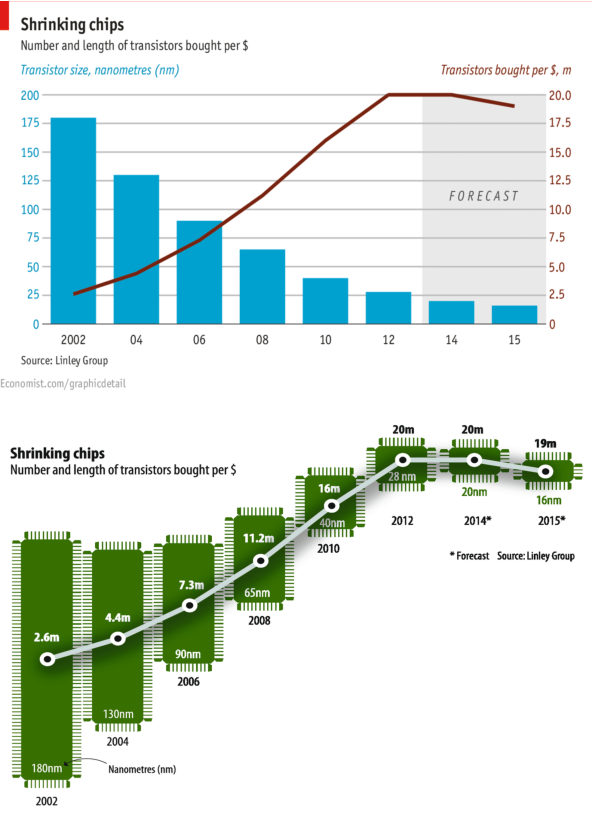
\includegraphics[width=0.30\textwidth, height=0.5\textwidth, valign=c]{img/moore.pdf}
		\vphantom{
			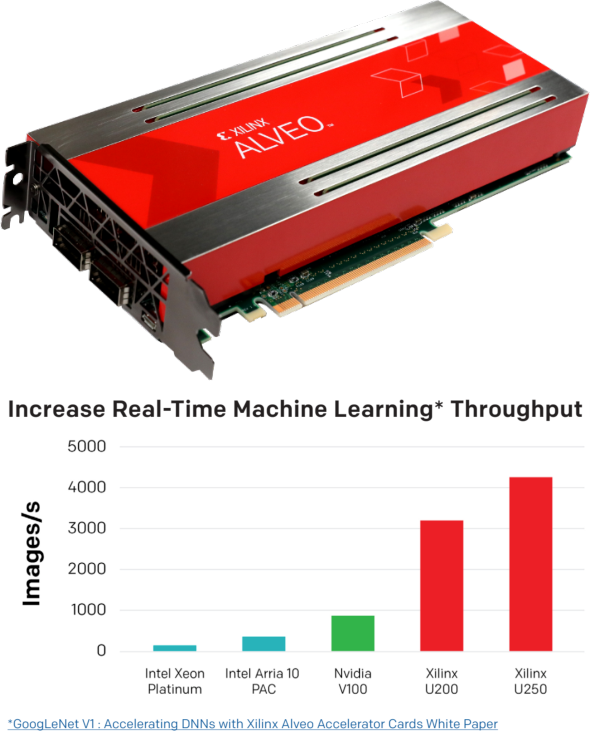
\includegraphics[width=0.30\textwidth, height=0.4\textwidth, valign=c]{img/alveo.pdf}
			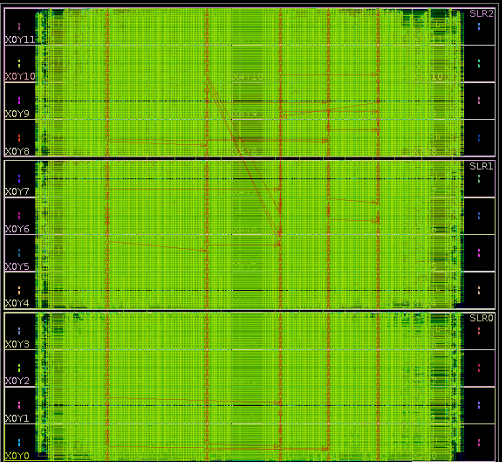
\includegraphics[width = 0.30\textwidth, height=0.5\textwidth, valign=c]{img/vivado-placed}
		}
	}
	\hfill
	\subfloat[Xilinx ALVEO FPGA]{
		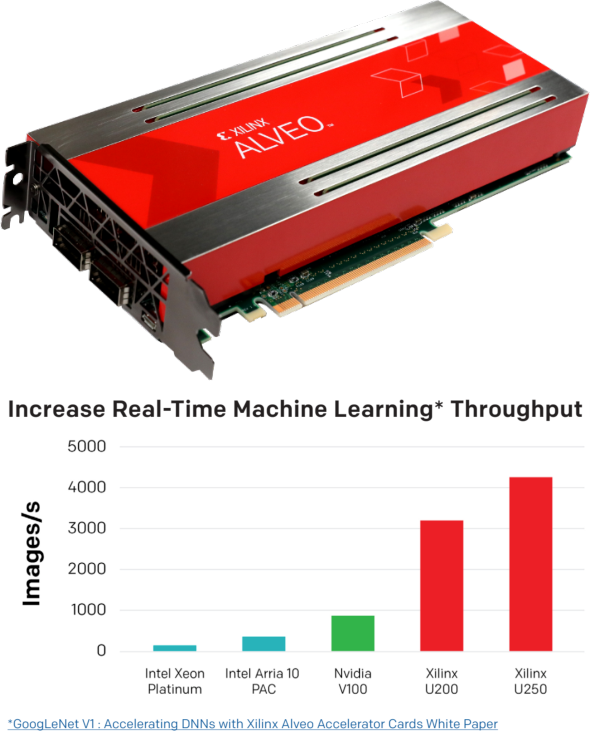
\includegraphics[width=0.30\textwidth, height=0.4\textwidth, valign=c]{img/alveo.pdf}
		\vphantom{
			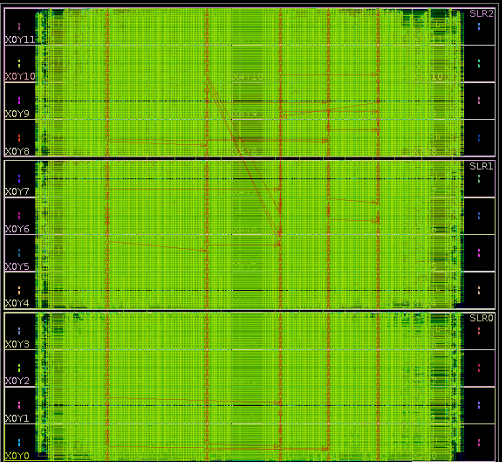
\includegraphics[width = 0.30\textwidth, height=0.5\textwidth, valign=c]{img/vivado-placed}
		}
	}
	\hfill
	\subfloat[Vivado fails routing]{
		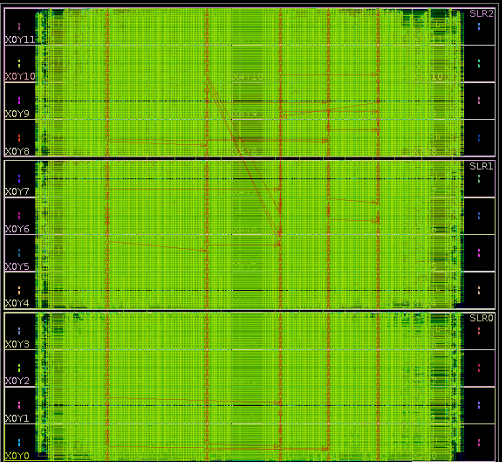
\includegraphics[width = 0.30\textwidth, height=0.5\textwidth, valign=c]{img/vivado-placed}
	}
	
	\caption{Current EDA tools are challenged by large high-density designs}
\end{figure}

\end{frame} 


% \begin{frame}{工作概述}

%   本毕业设计的目标与主要贡献为:

%   \begin{columns}[T, onlytextwidth]
%     \column{0.47\textwidth}

%     \vspace{0.5cm}

%     \begin{enumerate}
%       \setlength\itemsep{1.5em}
%       \item 解决大规模加速器设计布局难度大、时间成本高的问题;
%       \item 提出时间更短、性能更优的进化布局算法;
%       \item 构建端到端的自动FPGA布局布线框架:RapidLayout;
%       \item 提出布局结果的迁移学习方法。
%     \end{enumerate}

%     \column{0.5\textwidth}
%     % \begin{figure}
%     %   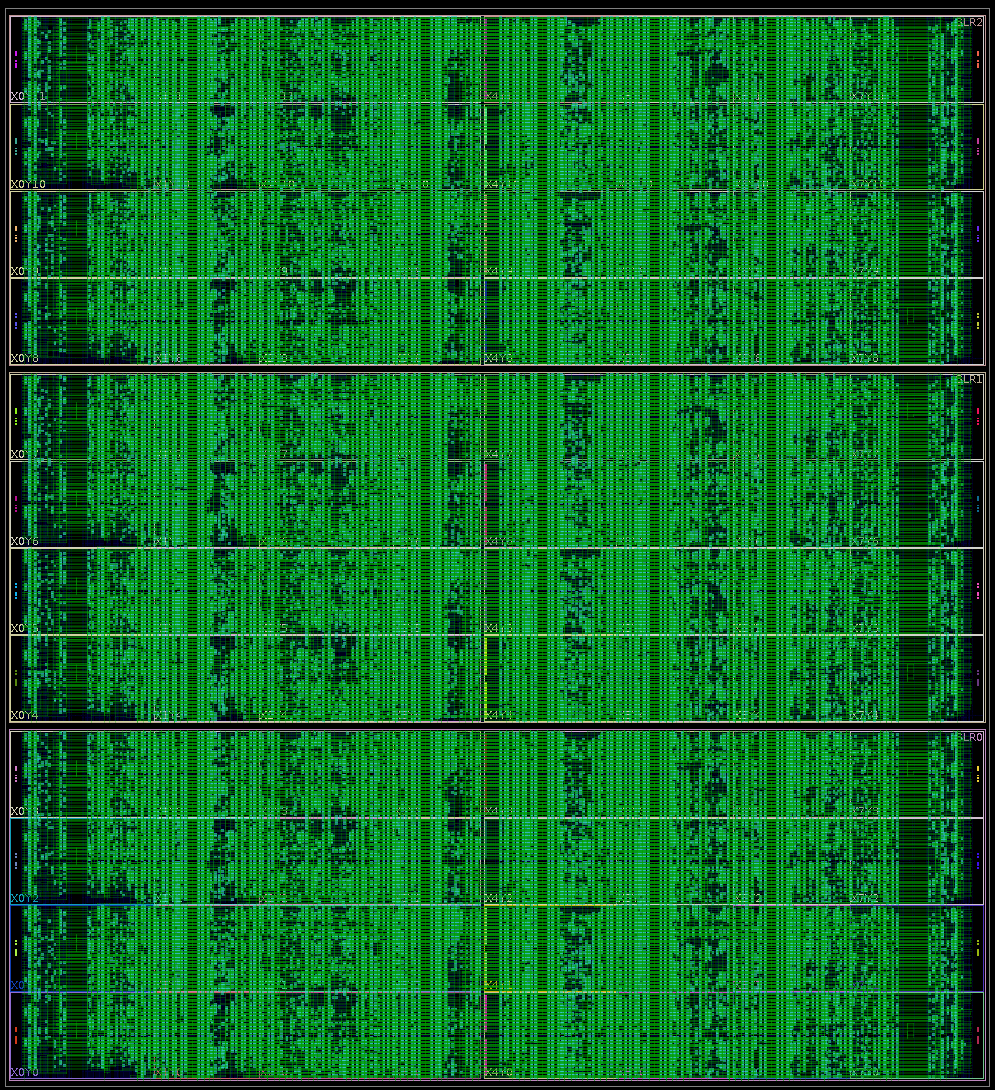
\includegraphics[width=1\textwidth,height=1.3\textwidth]{img/rapidlayout-placed}
%     %   \caption{使用RapidLayout完成布局布线的脉动阵列神经网络加速器}
%     % \end{figure}

%     \begin{figure}[h]
%       \centering
%       \subfloat[Vivado]{
%         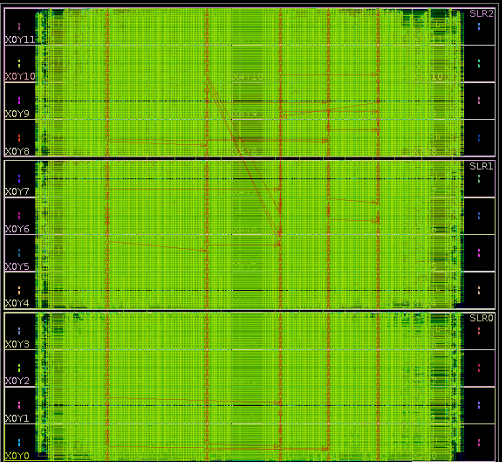
\includegraphics[width=0.5\textwidth, height=0.8\textwidth]{img/vivado-placed.png}
%       }
%       \subfloat[RapidLayout] {
%         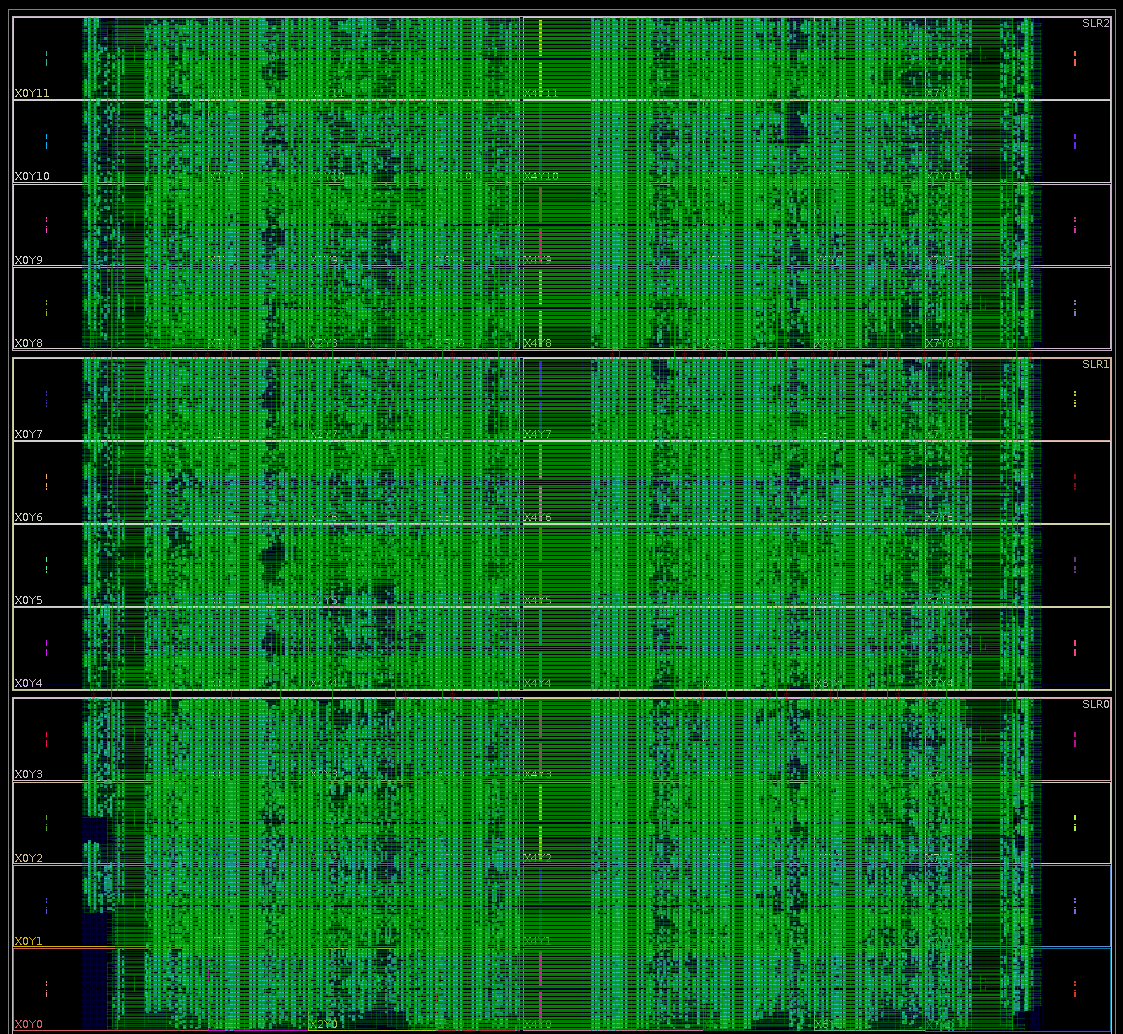
\includegraphics[width=0.5\textwidth, height=0.8\textwidth]{img/manual-placed.png}
%       }
%       \caption{
%        480核CNN加速器布局布线
%       }
%       \label{fig:overview}
%     \end{figure}


%   \end{columns}


% \end{frame}


% \section{相关技术概述}

\begin{frame}{FPGA Implementation and Placement Algorithms}

  \begin{columns}[T, onlytextwidth]
    \column{0.4\textwidth}

      \begin{figure}
        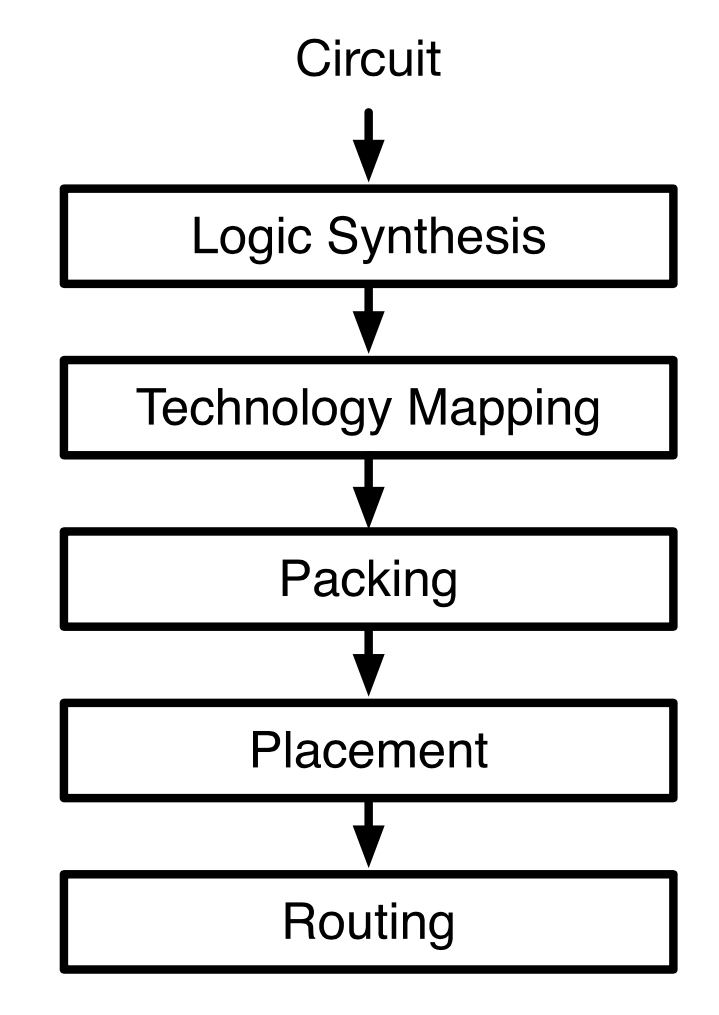
\includegraphics[width=0.8\textwidth]{img/cad.png}
      \end{figure}

    \column{0.6\textwidth}

      \begin{enumerate}
        \item Simulated Annealing
        \begin{itemize}
          \item Near optimal results
          \item Not scalable, hard to parallelize
        \end{itemize}
        \item Min-Cut
        \begin{itemize}
          \item Short runtime
          \item Likely to stuck in local optima
        \end{itemize}
        \item Analytic Placement
        \begin{itemize}
          \item State-of-the-Art
          \item Complex legalization
        \end{itemize}
        \item Evolutionary algorithms
        \begin{itemize}
          \item Inferior to SA
          \item Friendly to parallelism
        \end{itemize}
      \end{enumerate}

  \end{columns}

\end{frame}

\begin{frame}{RapidWright and Hard Blocks}

\begin{figure}
  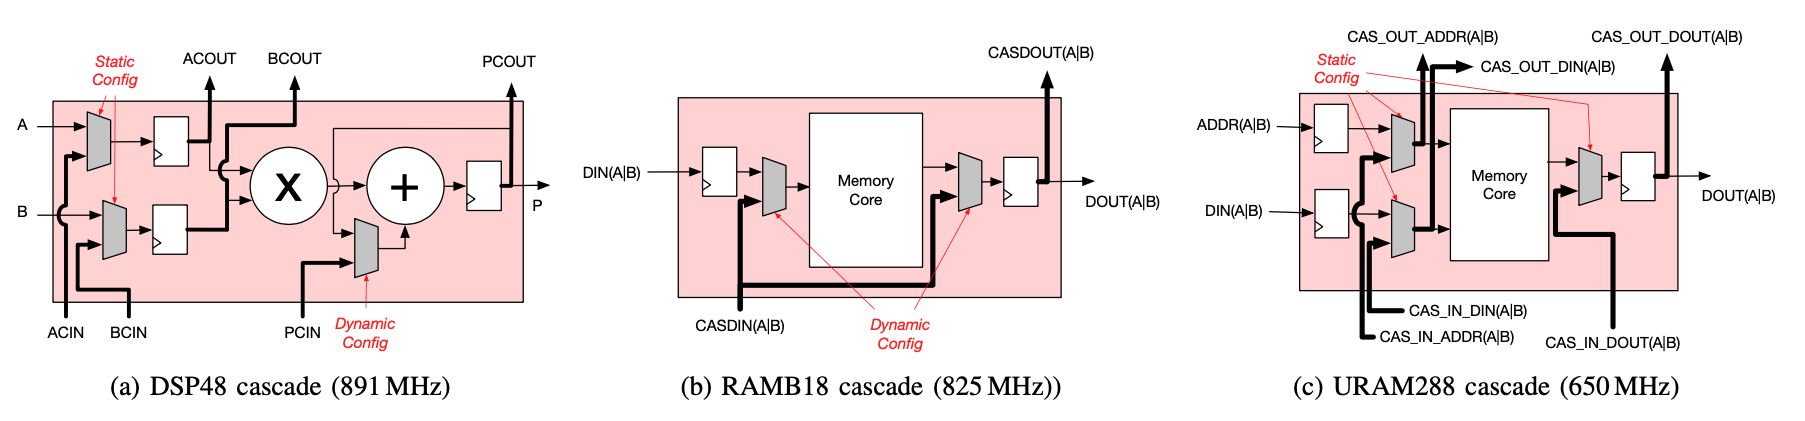
\includegraphics[width=1.0\textwidth]{img/hardblocks.png}
  \vspace{-0.3cm}
\end{figure}

\begin{columns}[T, onlytextwidth]
  \column{0.4\textwidth}
    \begin{figure}
      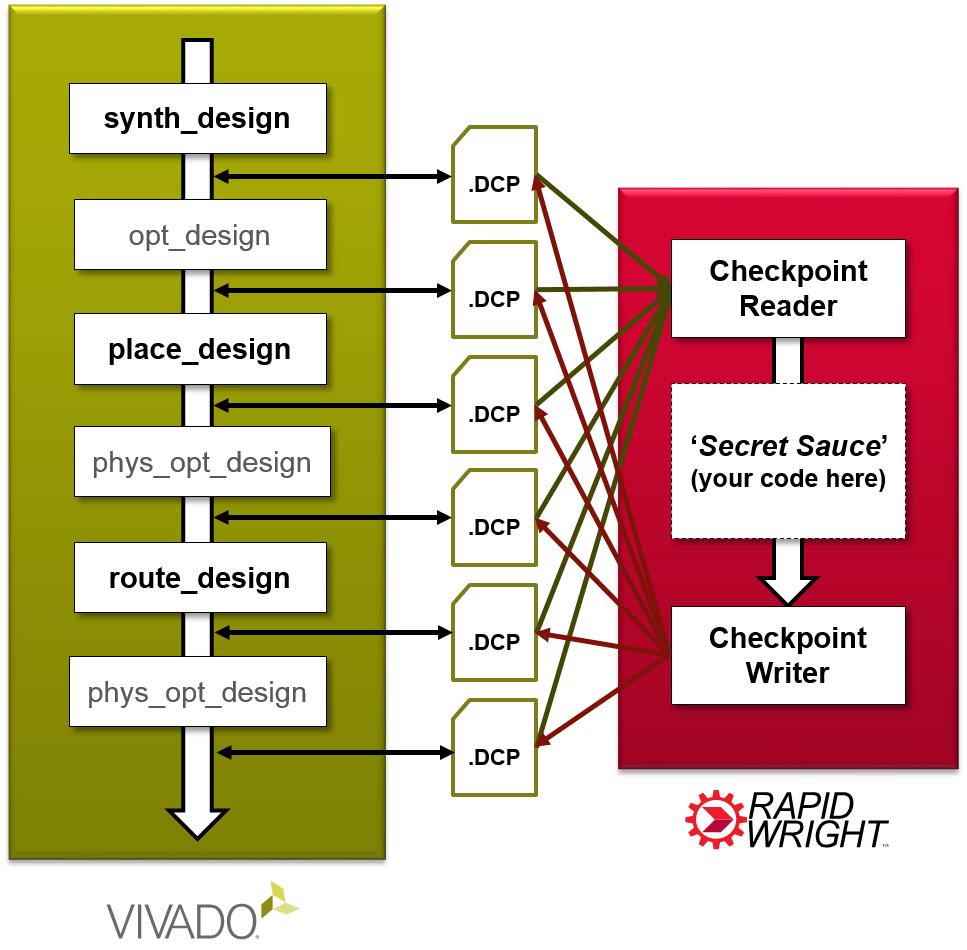
\includegraphics[width=\textwidth]{img/vivado_dcps.png}
    \end{figure}


  \column{0.55\textwidth}
    {\fontsize{7}{10}
    \emph{UltraScale+ Hard Blocks}
    \begin{itemize}
      \item {\bf DSP48E2:} 27$\times$18 Mult 48-bit Add
      \item {\bf RAMB18:} 18KB TDP/SDP, supporting \alert{cascade}
      \item {\bf URAM288:} 288KB, supporting \alert{cascade}
    \end{itemize}

    \emph{RapidWright FPGA framework}
    \begin{itemize}
      \item Read/Write DCP files 
      \item Modular design methods
      \item Logic/Physical netlist modification
      \item Fast access to physical information
    \end{itemize}
    }
  
\end{columns}

\end{frame}

\begin{frame}{Systolic Arrays and Evolutionary Algorithms}

  \begin{columns}[T, onlytextwidth]
  
    \column{0.5\textwidth}
    \begin{figure}
      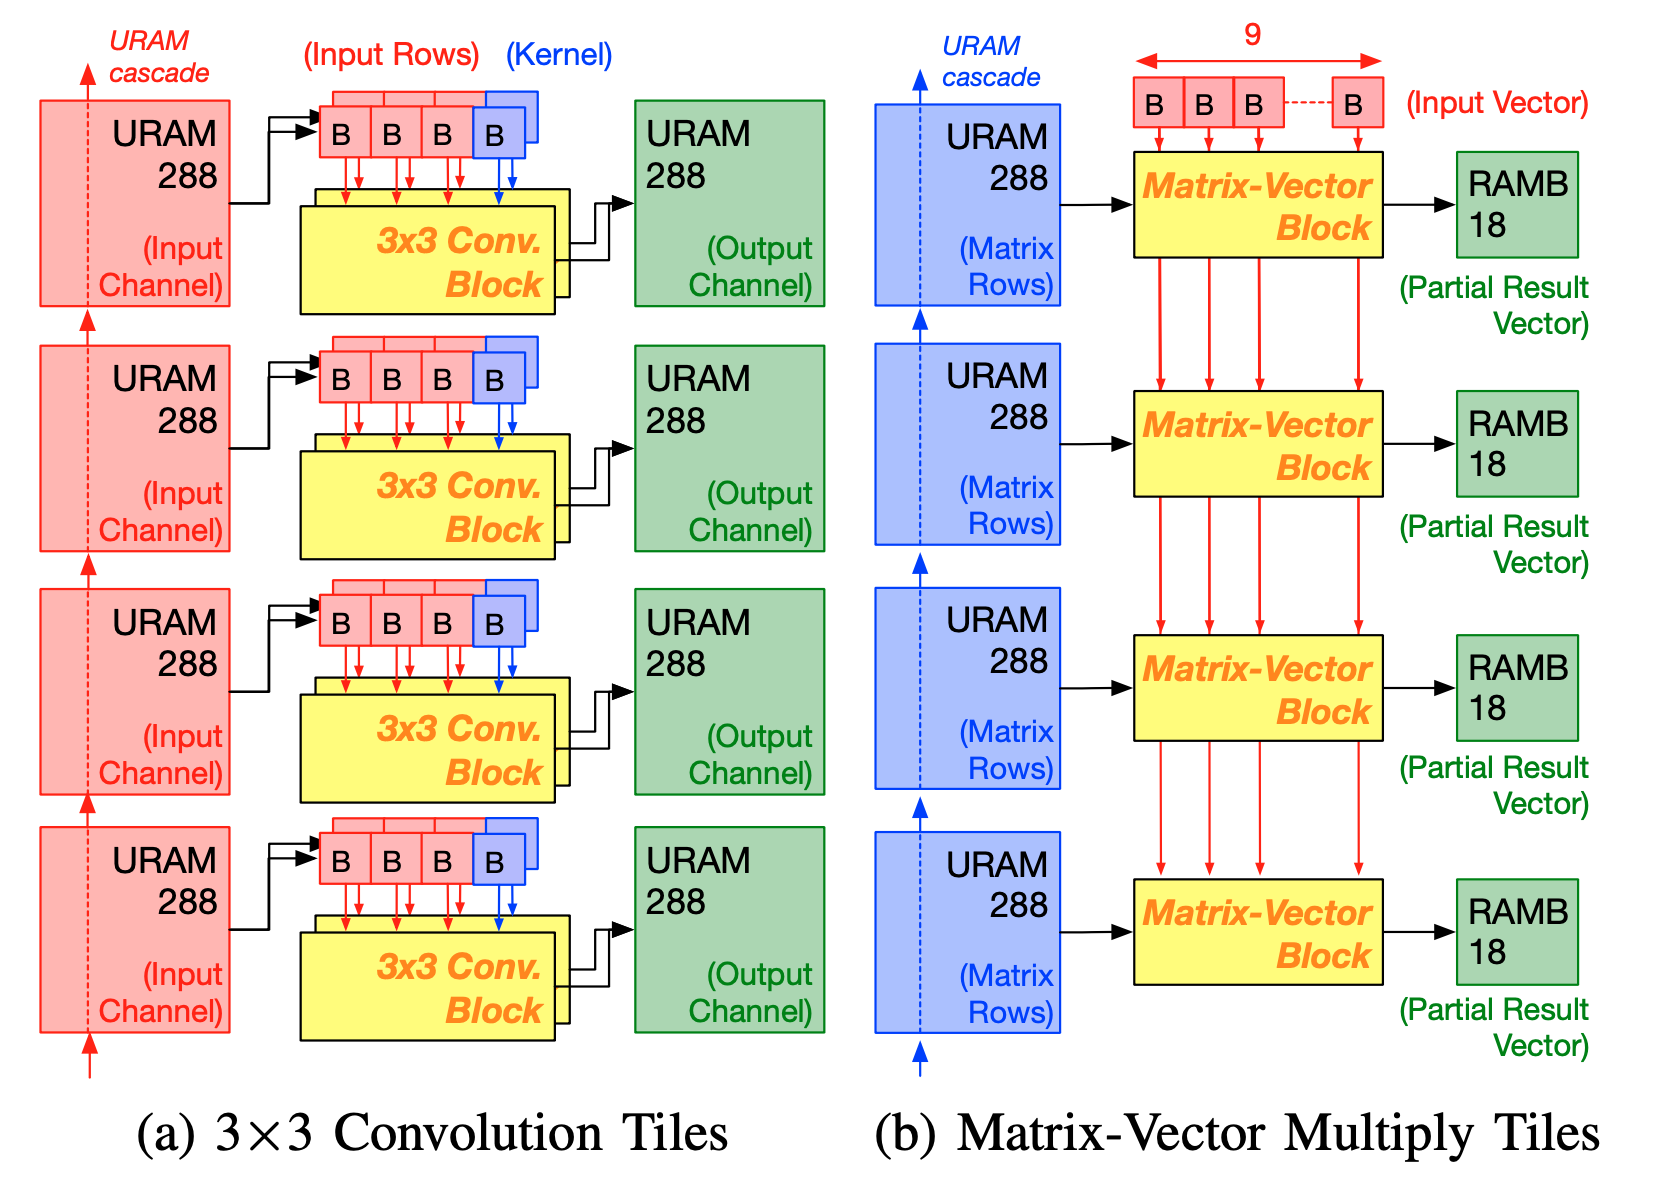
\includegraphics[width=\textwidth]{img/cascade.png}
      \vspace{-0.5cm}
    \end{figure}

    \begin{figure}
      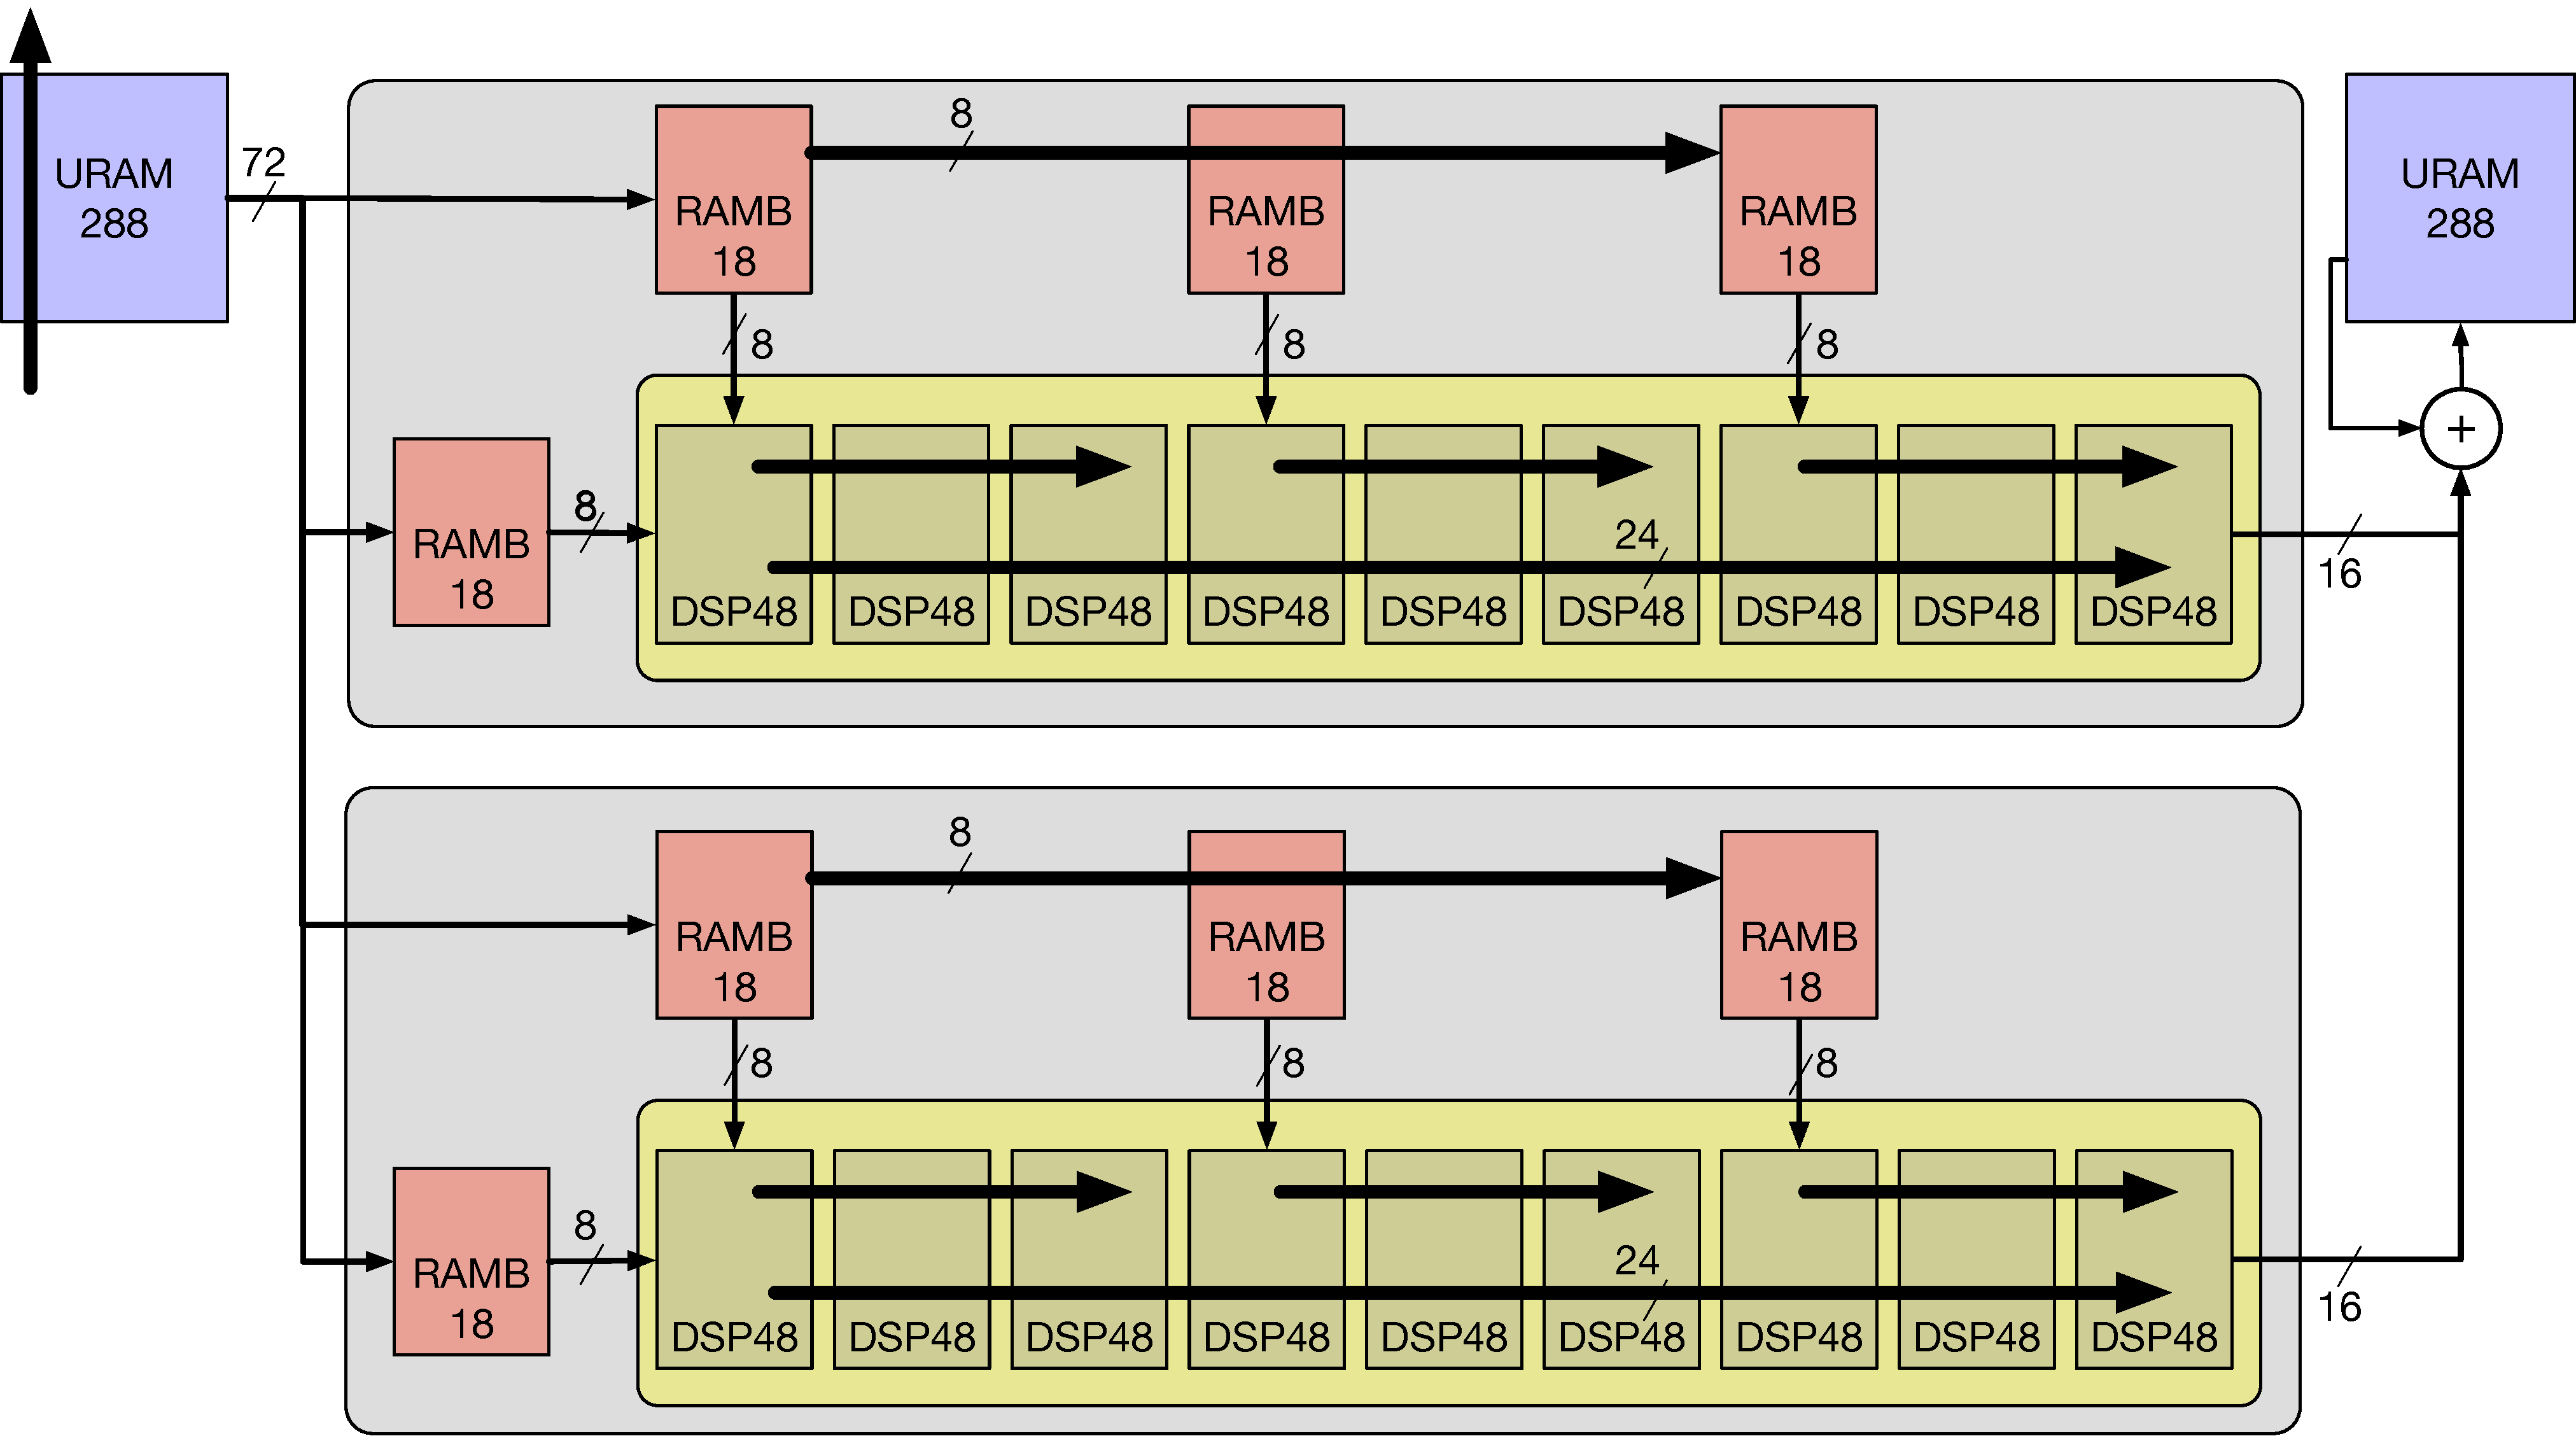
\includegraphics[width=0.8\textwidth]{img/array}
      \caption{Our systolic array design}
    \end{figure}
  
    \column{0.4\textwidth}
    \vspace{-0.2cm}
    \begin{center}
      \animategraphics[loop, controls, width=0.8\textwidth]{10}{img/cmaes/frame}{0}{19}
    \end{center}

    \vspace{-0.3cm}
    \begin{figure}
      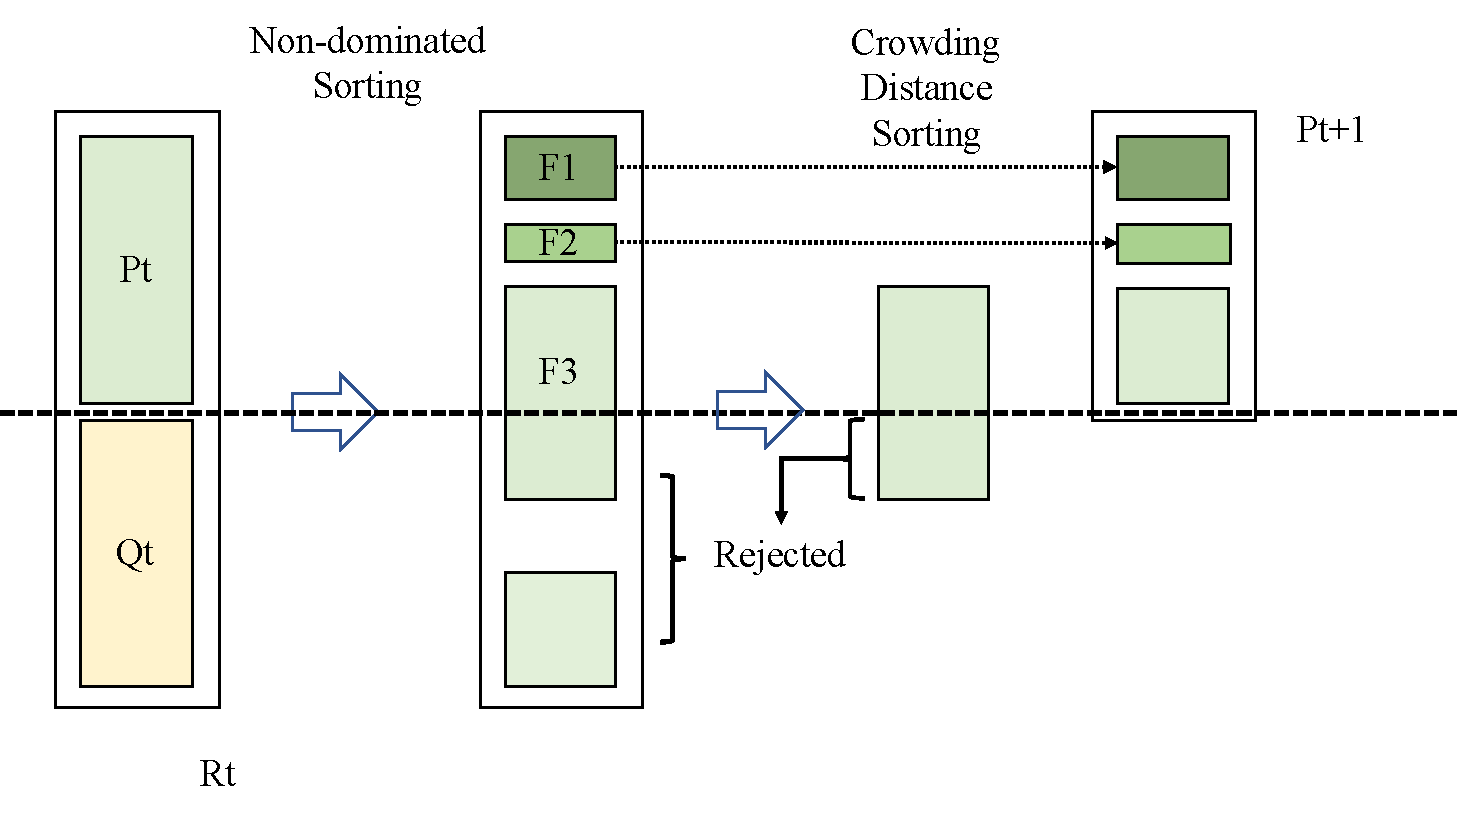
\includegraphics[width=\textwidth]{img/NSGA-II.pdf}
      \caption{CMA-ES and NSGA-II}
    \end{figure}

  \end{columns}

\end{frame}


\section{Evolutionary Hard Block Placement}

\begin{frame}{Problem Formulation}
  \vspace{-0.5cm}
  \begin{figure}
    \centering
    \resizebox{0.6\linewidth}{!}{
    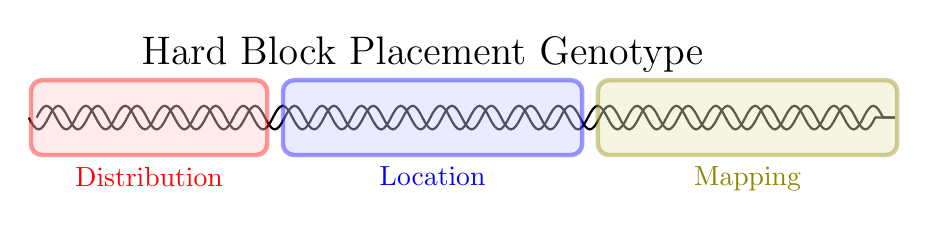
\begin{tikzpicture}[decoration={coil},
  dna/.style={decorate, thick, decoration={aspect=0, segment length=0.5cm}}]
   
  %DNA
    \draw[dna, decoration={amplitude=.15cm}] (.1,0) -- (11,0);
    \draw[dna, decoration={amplitude=-.15cm}] (0,0) -- (11,0);
    \node at (5,0.8) {\Large Hard Block Placement Genotype};
  
    \node [rectangle,rounded corners,inner sep=0pt,minimum width=3cm, minimum
    height=0.25cm,text height=0.95cm, draw=red, ultra thick, fill=red!20,
    anchor=west, opacity=0.4, text
    opacity=1,label=below:{\textcolor{red}{Distribution}}] at (0,0) {};
  
    \node [rectangle,rounded corners,inner sep=0pt,minimum width=3.8cm, minimum
    height=0.25cm,text height=0.95cm, draw=blue, ultra thick, fill=blue!20,
    anchor=west, opacity=0.4, text
    opacity=1,label=below:{\textcolor{blue}{Location}}] at (3.2,0) {};
   
  
    \node [rectangle,rounded corners,inner sep=0pt,minimum width=3.8cm, minimum
    height=0.25cm,text height=0.95cm, draw=olive, ultra thick, fill=olive!20,
    anchor=west, opacity=0.4, text
    opacity=1,label=below:{\textcolor{olive}{Mapping}}] at (7.2,0) {};
   
    \end{tikzpicture}
    
    }

    \vspace{-0.2cm}
    
    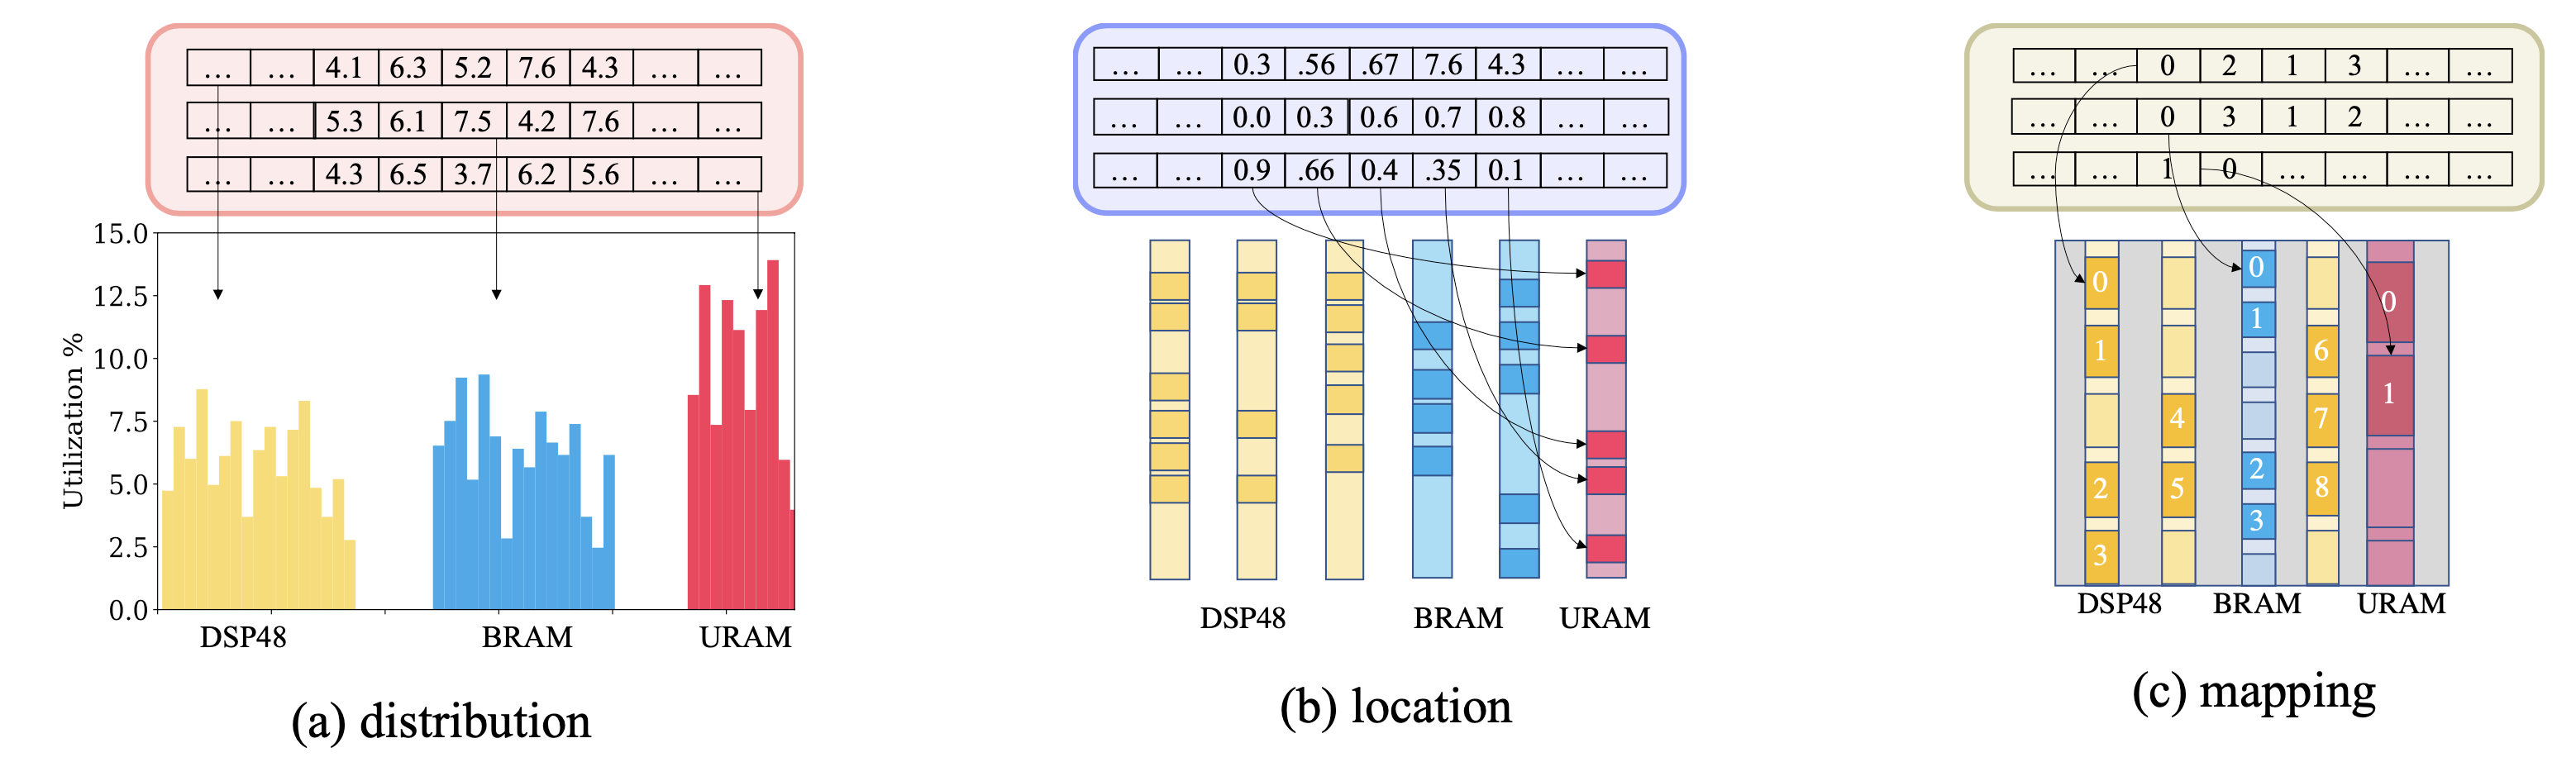
\includegraphics[width=\textwidth]{img/geno.png}
    
    \label{fig:genotype}
  \end{figure}

  \vspace{-0.3cm}

  {\fontsize{8}{10}
    \begin{columns}[T, onlytextwidth]

      \column{0.5\textwidth}

      {\small Minimize:} 
      \vspace{-0.3cm}
      \begin{equation} \label{eq:obj1}
        \vspace{-0.5cm}
        \sum_{i,j} ((\Delta{x_{i,j}} + \Delta{y_{i,j}}) \cdot w_{i,j})^2 
      \end{equation}
      
      \begin{equation} \label{eq:obj2}
        \max_{k} (BBoxSize(C_k))
        \vspace{-0.2cm}
      \end{equation}

      {\small subject to:}
      \vspace{-0.3cm}
      % rectangle region bound
      \begin{equation} \label{eq:region}
        \vspace{-0.5cm}
        0 \leq x_i < XMAX ,\ 
        0 \leq y_i < YMAX
      \end{equation}
      
      
     
      
      
      
      \column{0.46\textwidth}

      % no overlap
      \begin{equation} \label{eq:overlap}
        \vspace{-0.5cm}
          {x_i,y_i} \neq {x_j,y_j}
        \vspace{-0.2cm}
      \end{equation}

      % cascade connection placement requirement
      \begin{equation} \label{eq:cascade}
        \vspace{-0.5cm}
        \begin{aligned}[b]
        & \textrm{if block\ } i \textrm{ is cascaded after\ } j \textrm{ : }
        x_i = x_j \\
        & y_i =
        \begin{cases}
           y_j + 1  & i, j \in \{  DSP, URAM  \} \\
           y_j + 2  & i, j \in \{  RAMB \}
        \end{cases}
      \end{aligned}
      \end{equation}
      
    \end{columns}
  
  }
  
  
\end{frame} 


\begin{frame}{RapidLayout Workflow}

  \begin{columns}[T, onlytextwidth]
    \column{0.4\textwidth}

    \vspace{0.2cm}
    {\fontsize{7}{10}\selectfont

    \circled{A} {\bf Netlist Replication:}\\
    Takes one computation unit's logic netlist as input and finds the \alert{minimum replicating rectangle}
    and replicate the logic netlist.\\

    \circled{B} {\bf Evolutionary Placement:}\\
    Solves the placement problem with NSGA-II or CMA-ES.\\

    \circled{C} {\bf Placement and Site Routing:}\\
    Embedsthe placement result into DCP checkpoint.\\

    \circled{D} {\bf Post-Placement Pipelining:}\\
    Determines pipeline depth based on wirelength.\\

    \circled{E} {\bf SLR Placement and Routing:}\\
    Calls Vivado to finish routing of 1 SLR. \\

    \circled{F} {\bf SLR Replication:}\\
    Replicates the routed design to fill the FPGA.\\

    }

    \column{0.5\textwidth}

    % figure: design flow
    
    \tikzstyle{block} = [thick, rectangle, draw, fill=white, text width=12em, text centered, rounded corners, minimum height=2em]
    \tikzstyle{invisiblock} = [rectangle, fill=white, text width=12em, text centered, rounded corners, minimum height=2em]
    \tikzstyle{decisionblock} = [rectangle, draw, fill=blue!20, text width=12em, text centered, rounded corners, minimum height=2em]
    \tikzstyle{line} = [draw, -latex']
    
    \pgfdeclarelayer{bg}    % declare background layer
    \pgfsetlayers{bg,main}  % set the order of the layers (main is the standard layer)
  
    \begin{figure}
    \begin{center}
    \scalebox{0.5}{
    \begin{tikzpicture}[node distance=1.5cm and 3.5cm, scale=1, transform shape]
      % Place nodes
      \node [invisiblock] (input) {Convolution Block DCP};
      \node [block, below of=input] (replicate) {Netlist Replication {\bf [\textless 1s]}};
      \circledat{A}{replicate.north west};
      \node [block, below of=replicate, minimum height=7em, node distance=2.5cm] (evolve) {Evolutionary\\ Hard Block\\ Placement\\ {\bf [30\,s--5\,min]}};
      \circledat{B}{evolve.north west};
      \node [block, below of=evolve, node distance=2.5cm] (siteroute) {Placement and\\ Site Routing {\bf [$\approx$3\,min]}};
      \circledat{C}{siteroute.north west};
      \node [block, below of=siteroute] (pipeline) {Post-Placement\\Pipelining {\bf [$\approx$10\,s]}};
      \circledat{D}{pipeline.north west};
      \node [block, below=0.75cm of pipeline] (vivado) {SLR Placement\\ and Routing {\bf [$\approx$54\,min]}};
      \circledat{E}{vivado.north west};
      \node [block, below=0.75cm of vivado] (slr) {SLR Replication {\bf [$\approx$2\,min]}};
      \circledat{F}{slr.north west};
      % Draw sub-nodes
        \node [block, fill=teal!50, right=1cm of evolve] (two) {Compute objective};
      \node [block, fill=teal!50, above of=two] (one) {Generate candidates};
      \node [block, fill=teal!50, below of=two] (three) {Update};
      % Inner loop highlight
      \begin{pgfonlayer}{bg}
      
      \path[rounded corners, draw=blue, thick, fill=blue!10,opacity=0.9] 
      ([xshift=-0.75em,yshift=0.75em]vivado.north west) to ([xshift=10em,yshift=0.75em]vivado.north east) 
      to ([xshift=10em,yshift=-0.75em]vivado.south east) to ([xshift=-0.75em,yshift=-0.75em]vivado.south west) -- cycle;
      
      
      \path[rounded corners, draw=red, thick, fill=red!10,opacity=0.9] 
      ([xshift=-0.75em,yshift=0.75em]replicate.north west) to 
    ([xshift=20em,yshift=0.75em]replicate.north east) to 
    ([xshift=20em,yshift=-0.75em]slr.south east) to
    ([xshift=-0.75em,yshift=-0.75em]slr.south west) to
    ([xshift=-0.75em,yshift=0.75em]slr.north west) to 
    ([xshift=12em,yshift=0.75em]slr.north east) to
      ([xshift=12em,yshift=-0.75em]pipeline.south east) to 
    ([xshift=-0.75em,yshift=-0.75em]pipeline.south west) -- cycle;
      
      \path[rounded corners, draw=teal, thick, fill=teal!10,opacity=0.9] 
      ([xshift=-0.5em,yshift=0.5em]evolve.north west) to ([xshift=0.5em,yshift=0.5em]evolve.north east) 
      to ([xshift=-0.5em,yshift=1.5em]one.north west) to ([xshift=3.5em,yshift=1.5em]one.north east) 
      to ([xshift=3.5em,yshift=-1.5em]three.south east) to ([xshift=-0.5em,yshift=-1.5em]three.south west) 
      to ([xshift=0.5em,yshift=-0.5em]evolve.south east) to ([xshift=-0.5em,yshift=-0.5em]evolve.south west) -- cycle;
      \end{pgfonlayer}
      
      %\node [draw=none,below right=0.1cm of three] (opt4j) {\bf Opt4J};
      \node [draw=none,right=3.5cm of slr] (RapidWright) {\Large \bf RapidWright};
      \node [draw=none,right=1.75cm of vivado] (RapidWright) {\Large \bf Vivado};
      
      \node [invisiblock,below of=slr] (output) {Bitstream};
      % Draw edges
      \path [line, thick] (input) -- (replicate);
      \path [line, thick] (replicate) -- (evolve);
      \path [line, thick] (evolve) -- (siteroute);
      \path [line, thick] (siteroute) -- (pipeline);
      \path [line, thick] (pipeline) -- (vivado);
      \path [line, thick] (vivado) -- (slr);
      \path [line, thick] (slr) -- (output);
      % Draw sub-edges
      \path [line, thick] (one) -- (two);
      \path [line, thick] (two) -- (three);
      % Loops
      \path [line, thick] (three.east) -- ([xshift=0.8cm]three.east) -- ([xshift=0.8cm]one.east) node [midway, above, sloped, rotate=180] (textnode0) {evolve} -- (one.east);
    
    \end{tikzpicture}
    }
    \end{center}
    % 	\caption{RapidLayout Design Flow with runtime details for the Xilinx VU11P
    %  FPGA along with tool usage information. Bulk of the intelligent exploration is done in RapidWright, and Vivado is only invoked at the end for final placement and routing.}
    
    \caption{RapidLayout Workflow}
    
    \label{fig:flow}
    \vspace{-0.1in}
    \end{figure}

  \end{columns}

\end{frame}


\begin{frame}{Example: Xilinx UltraScale+ VU11P}

  \begin{columns}[T, onlytextwidth]

    \column{0.5\textwidth}
    \vspace{-0.5cm}
    \begin{figure}
      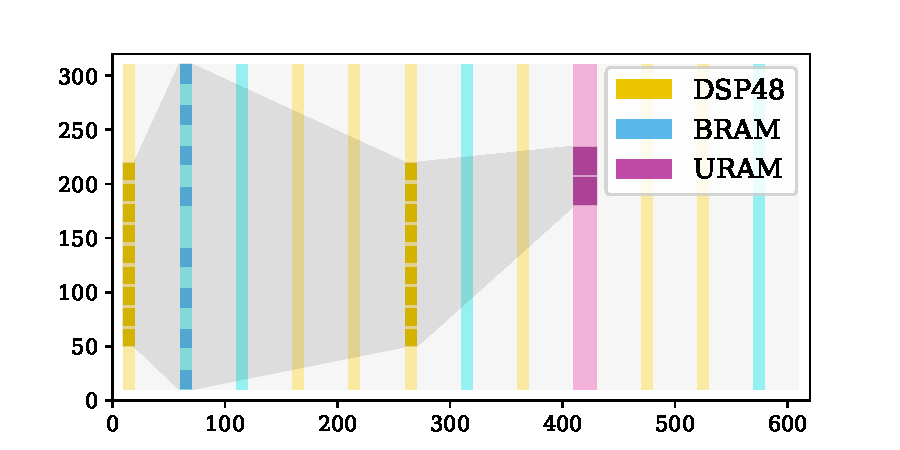
\includegraphics[width=\textwidth]{img/block1}
      \caption{1 convlution unit}
    \end{figure}
    \vspace{-1cm}
    \begin{figure}
      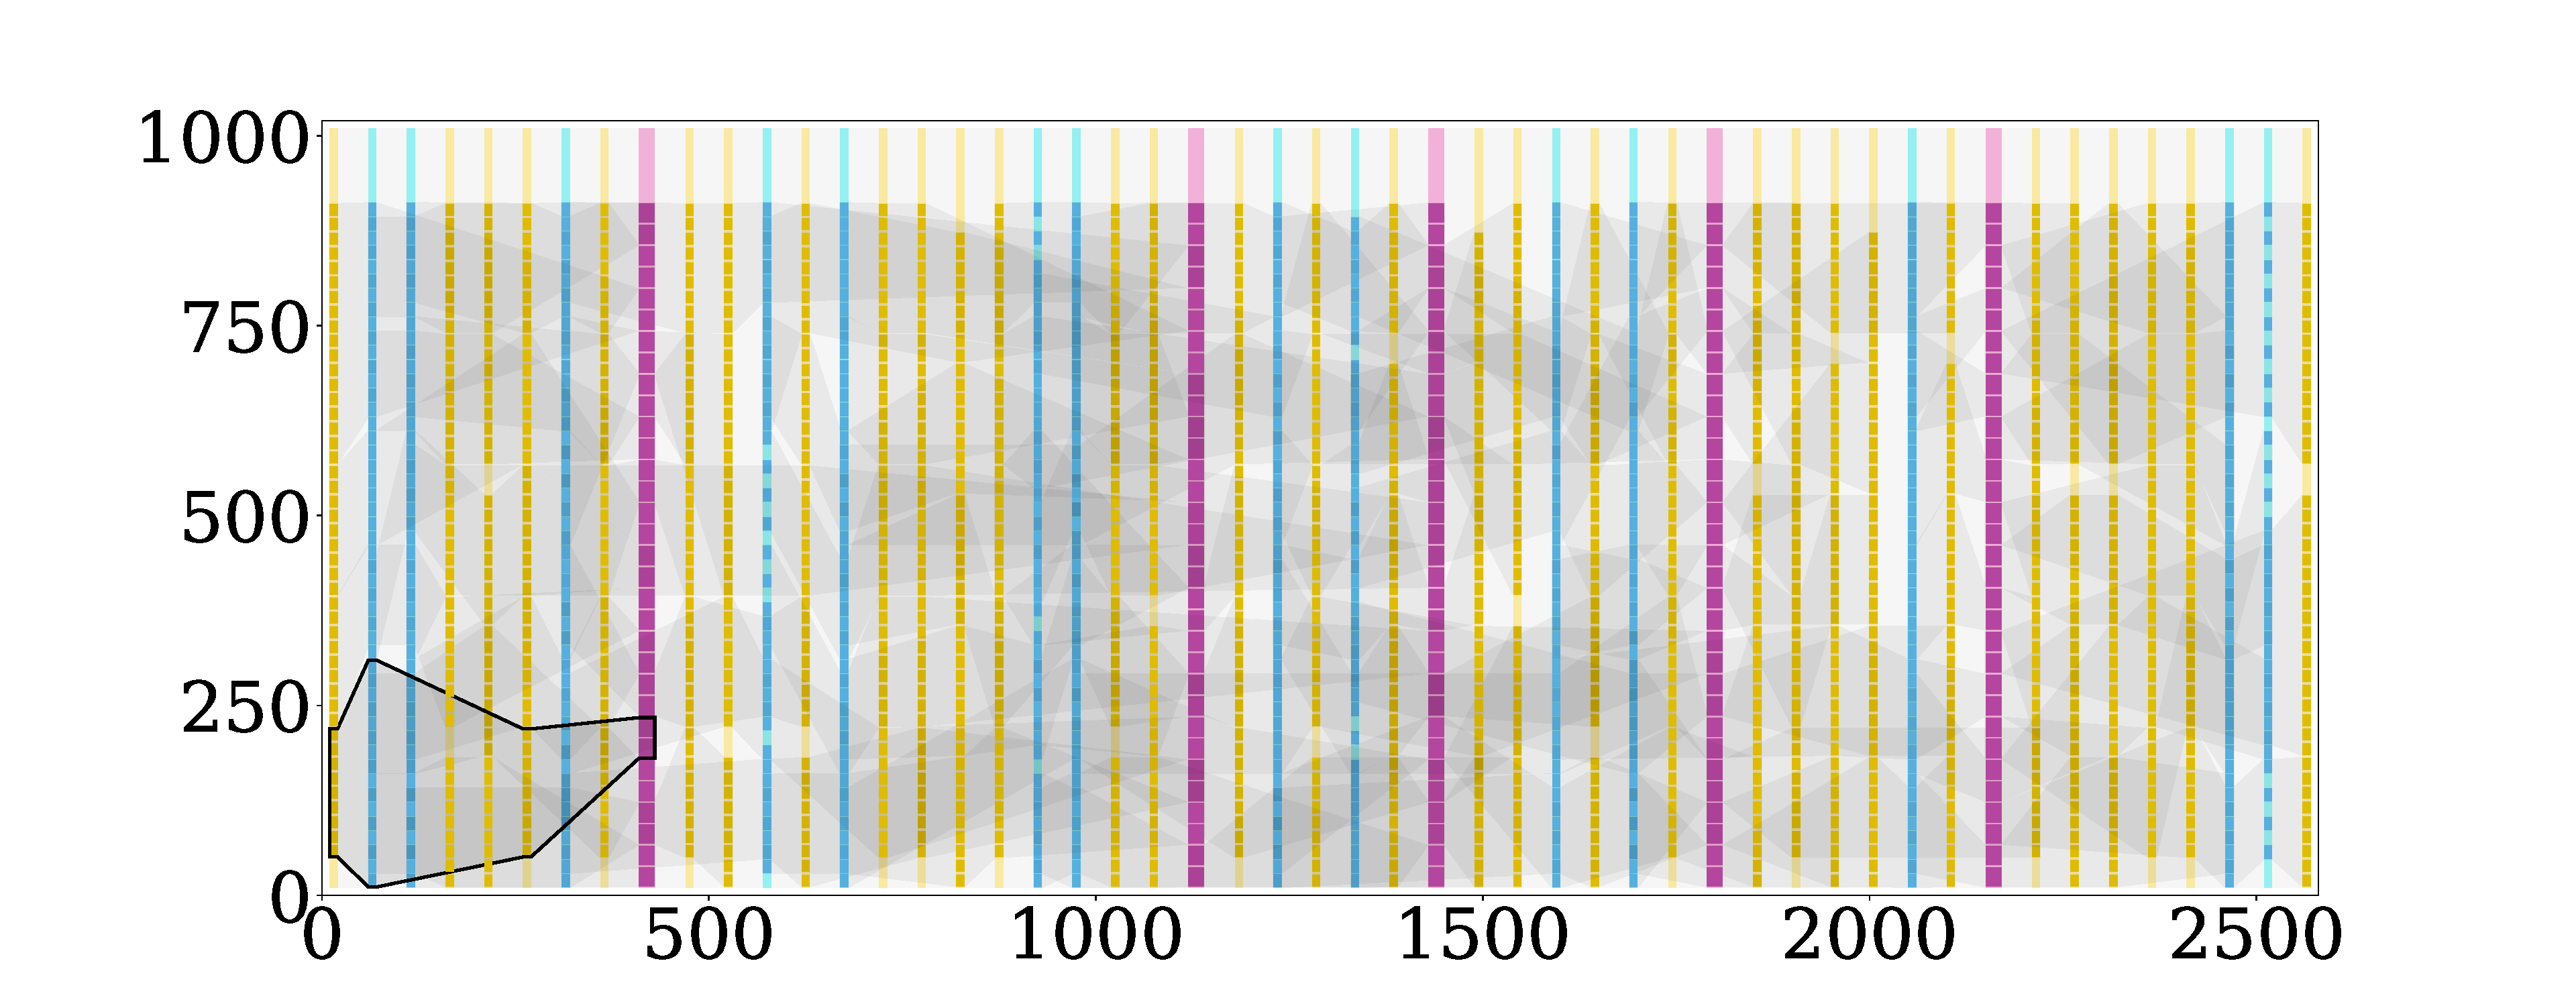
\includegraphics[width=\textwidth]{img/block80}
      \caption{Minimum Replicating Rect}
      \label{fig:block80}
    \end{figure}

    \column{0.5\textwidth}
    \begin{figure}
      \centering	
      \scalebox{0.8}{%
       \begin{tikzpicture}
       \centering
         \pgftext{%
           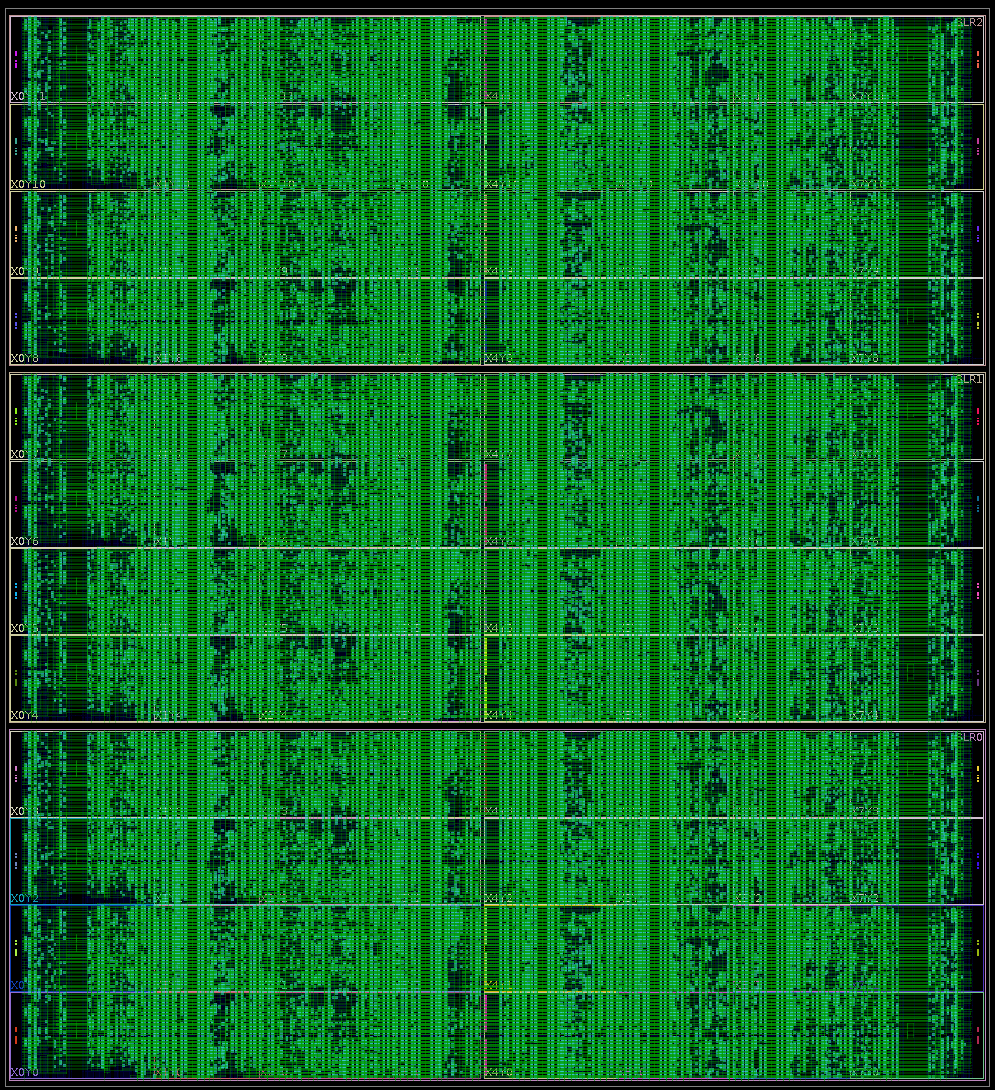
\includegraphics[width=0.78\textwidth]{img/rapidlayout-placed.png}
         }%
         \node [rectangle,rounded corners,minimum width=4.1cm,minimum
         height=0.7cm,draw=green,ultra thick,anchor=south west] (rect1) at
         (0.1-2.2,0.75-2.25) {};
         \node [rectangle,rounded corners,minimum width=4.2cm,minimum
         height=1.5cm,draw=red,ultra thick,anchor=south west,
         text=white,text opacity=0.5] (slr0) at
         (0.05-2.2,0-2.25) {\Huge SLR0};
         \node [rectangle,rounded corners,minimum width=4.1cm,minimum
         height=0.7cm,fill=green,opacity=0.5,draw
         opacity=1,draw=green,ultra thick,anchor=south
         west,text=black,text opacity=1,align=center] (rect0) at
         (0.1-2.2,-2.25+0.05) {Repeat Rect. (Fig~\ref{fig:block80})};
         \node [rectangle,rounded corners,minimum width=4.2cm,minimum
         height=1.5cm,draw=red,ultra thick,anchor=south west,
         text=white,text opacity=0.5] (slr1) at
         (0.05-2.2,1.5-2.25) {\Huge SLR1};
         \node [rectangle,rounded corners,minimum width=4.2cm,minimum
         height=1.5cm,draw=red,ultra thick,anchor=south west,
         text=white,text opacity=0.5] (slr2) at
         (0.05-2.2,3-2.25) {\Huge SLR2};
         \draw [ultra thick,->,green] (rect0) to [out=0,in=0,looseness=2] node (b)
       [midway,above=0cm,align=center,rotate=-90] {\textcolor{green}{{\small Copy Placements}
       }\textcolor{green}{{\small \ }}} (rect1);
       \draw [ultra thick,->,red] (slr0) to [out=180,in=180] node (a)
       [midway,above,align=center,rotate=90] {\textcolor{red}{{\small Copy Placement +
       Routing}}\\\textcolor{red}{{\small in RapidWright}}} (slr2);
         \circledat{F}{[yshift=2cm,xshift=0.35cm]a};
         \circledat{C}{[yshift=1cm,xshift=0.75cm]b};
         \circledat{D}{[yshift=0.0cm,xshift=0.75cm]b};
         \circledat{E}{[yshift=-1cm,xshift=0.75cm]b};
         \draw [ultra thick,->,red] (slr0) to [out=180,in=180] (slr1);
       \end{tikzpicture}
      }
      \caption{Placement \& SLR re-use}
      
    \end{figure}


  \end{columns}
  {\fontsize{8}{10}
  \begin{itemize}
    \item RapidLayout accelerates the end-to-end workflow by \alert{5--6 $times$} against Vivado
    \item Eliminates the long-period manual effort of trail-and-error
    \item High quality placement results and pipelining achieves \alert{650~MHz+} clock frequency
  \end{itemize}
  }
    
\end{frame}



%------------------------Spherical Interpolation Method-------------------------------
\section{Experiment Results}

\begin{frame}{QoR Comparison}
  
  \begin{columns}[T, onlytextwidth]

    \column{0.4\textwidth}

    {\fontsize{7}{10}\selectfont
      - Optimized Simulated Annealing\\
      - Verilog-to-Place-and-Route (VPR)\\
      - UTPlaceF \\
      - Single-objective Genetic Algorithm\\
      - Manual Placement\\
  
    }
    \vspace{0.3cm}
    %\begin{figure*}
      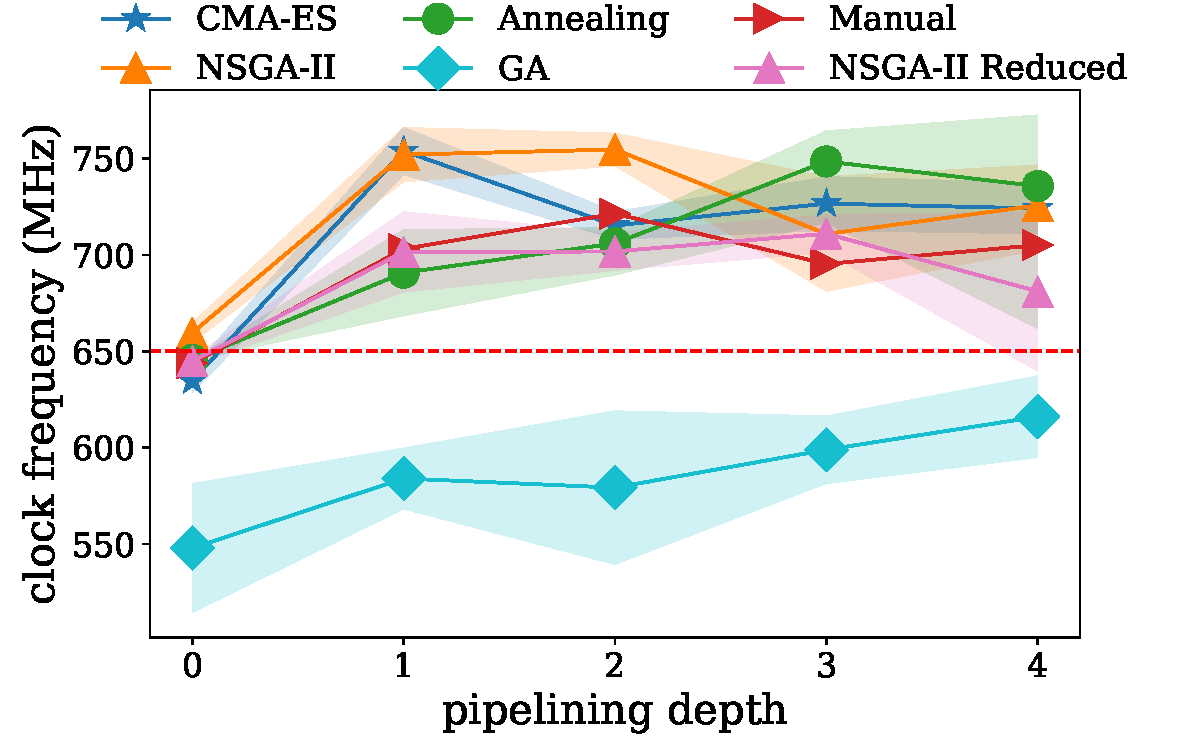
\includegraphics[width=\textwidth]{img/frequency_depth}
      %\caption{Freq. vs Depth}
    %\end{figure*}

    \column{0.6\textwidth}
    \vspace{-0.1cm}
    %\begin{figure*}
      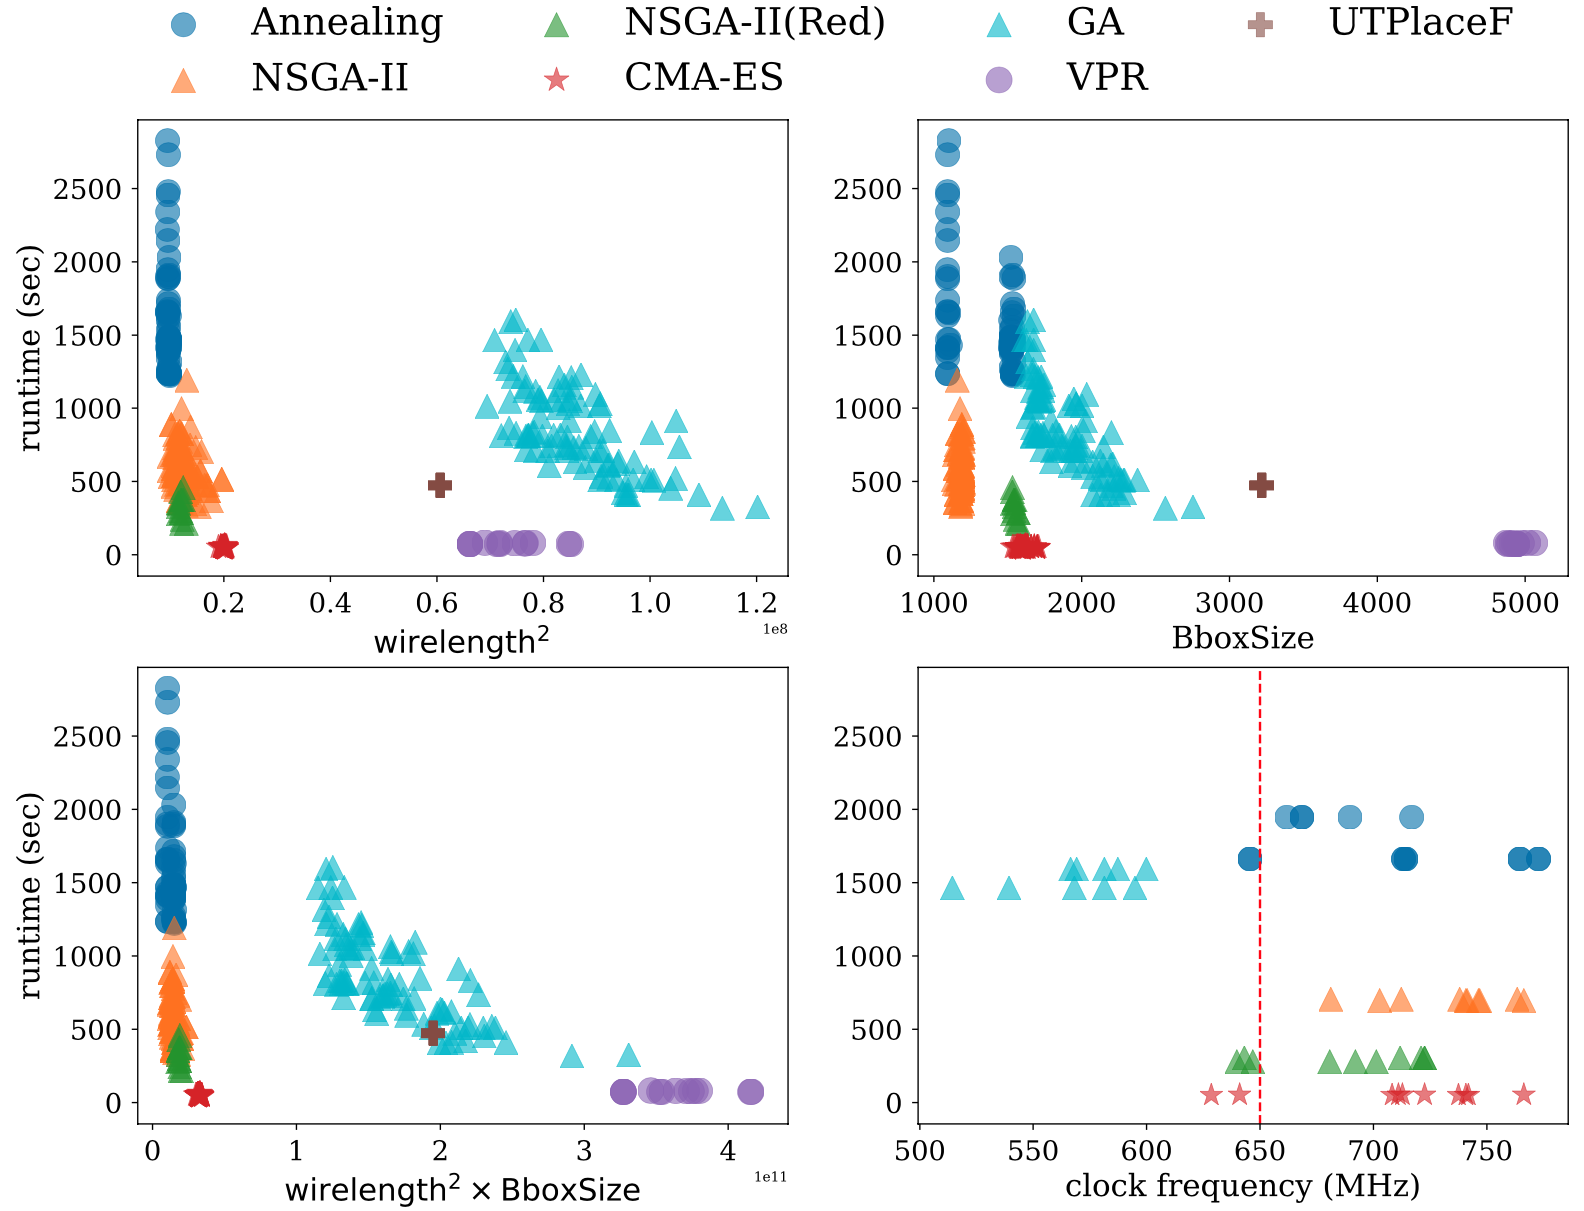
\includegraphics[width=1\textwidth]{img/objective-runtime.png}
      %\caption{Wirelength, BBox Size, and Frequency} 
      %\label{fig:objective}
    %\end{figure*}

  \end{columns}

  % \vspace{-0.2cm}


  {\fontsize{8}{12}\selectfont

  {\bf Conclusions:}\\
  \begin{enumerate}
    \item EA speeds up runtime over SA by \alert{2.7--30.8$\times$}
    \item EA wins wirelength over UTPlaceF and VPR by \alert{1.8--2.4$\times$}, bbox size by \alert{2.0--4.1$\times$}
    \item EA achieves 750~MHz high freq. with 1--2 level of pipelining,NSGA-II saves $\approx$17K(6\%) registers
  \end{enumerate}
  }

  % \vspace{-1.0cm}



  % \begin{table}
  %       % \caption{平均运行时间,平均线长,平均最大边界框尺寸,达到650MHz最少所需流水线寄存器数目,以及平均时钟频率对比。
  %       % 左侧为本文提出的NSGA-II, NSGA-II Reduced, CMA-ES,右侧为对比算法。与各个对比算法相比每个指标的提升倍数在
  %       % 括号内标出,其中\textcolor{red}{红色}$\rightarrow$NSGA-II,\textcolor{olive}{绿色}$\rightarrow$CMA-ES}
  %     \label{table:comparison}
  %     \centering
  %     \begin{adjustbox}{width=1.1\textwidth,center}
  %     \begin{tabular}{c|c c| c c c c c}
  %     \toprule
  %     Method             & NSGA-II    	          & CMA-ES       & SA 					                                                                       & GA 			                                                                  & VPR     	                                                                & UTPlaceF 		                                                                   &  Manual \\
  %     \midrule
  %     Runtime (secs)     & 586 (323)		          & 51  		     &1577     (\textcolor{red}{2.7$\times$}, \textcolor{olive}{30.8$\times$})		        & 850 (\textcolor{red}{1.5$\times$}, \textcolor{olive}{16.7$\times$})		      & 76 (\textcolor{red}{0.13$\times$}, \textcolor{olive}{1.5$\times$})		    &  473 (\textcolor{red}{0.8$\times$}, \textcolor{olive}{9.3$\times$})            & 1--2 wks\\
  %     Wirelength  	     & 3.5K  (3.5K)   		    & 4.4K     		 &3.1K 	   (\textcolor{red}{0.9$\times$}, \textcolor{olive}{0.7$\times$})		          & 9.2K  (\textcolor{red}{2.6$\times$}, \textcolor{olive}{2.1$\times$})    		& 8.5K (\textcolor{red}{2.4$\times$}, \textcolor{olive}{1.9$\times$})   		&  7.8K  (\textcolor{red}{2.2$\times$}, \textcolor{olive}{1.8$\times$})          & 8.1K (\textcolor{red}{2.3$\times$}, \textcolor{olive}{1.8$\times$})  \\
  %     BBox      	       & 1183  (1543)   		    & 1606     		 &1387	   (\textcolor{red}{1.2$\times$}, \textcolor{olive}{0.9$\times$})		          & 1908  (\textcolor{red}{1.6$\times$}, \textcolor{olive}{1.2$\times$})   		  & 4941	(\textcolor{red}{4.1$\times$}, \textcolor{olive}{3.1$\times$})  		&   3218	(\textcolor{red}{2.7$\times$}, \textcolor{olive}{2.0$\times$})         & 1785 (\textcolor{red}{1.5$\times$}, \textcolor{olive}{1.1$\times$})  \\
  %     Pipeline Reg.		   & 256K  (273K) 		      & 273K	   		 &273K	   (\textcolor{red}{1.1$\times$}, \textcolor{olive}{1$\times$}) 	 	          & 323K	(\textcolor{red}{1.3$\times$}, \textcolor{olive}{1.2$\times$})   		  & -		                                                                      &   -                                                                            & 306K (\textcolor{red}{1.2$\times$}, \textcolor{olive}{1.1$\times$})   \\
  %     Frequency	(MHz)	 	 & 733  (688)   & 708 	 &711  (\textcolor{red}{0.97$\times$}, \textcolor{olive}{1.0$\times$})		        & 585 	(\textcolor{red}{0.80$\times$}, \textcolor{olive}{0.83$\times$})	& - 	      	                                                              & - 	                                                                           & 693 (\textcolor{red}{0.95$\times$}, \textcolor{olive}{0.98$\times$}) \\
  %     \bottomrule
  %     \end{tabular}
  %   \end{adjustbox}
  % \end{table}

  % {\fontsize{7}{10}\selectfont
  %  括号内为指标提升倍数,其中\textcolor{red}{红色}$\rightarrow$NSGA-II,\textcolor{olive}{绿色}$\rightarrow$CMA-ES
  % }

\end{frame}


\begin{frame}{Transfer Learning}
  %\vspace{-2cm}

  \begin{table}[h!]
    \caption{Transfer Learning Performance: VU3P, VU11P as seed devices}
    \label{table:port}
    \centering
    \begin{adjustbox}{width=\columnwidth,center}
    \begin{tabular}{c|c c c c c}
      \toprule
  \multirow{2}{*}{Device}     & Design Size 		& Impl.Runtime 		& Frequency 	 & \multicolumn{2}{c}{Placement Runtime}    			\\ \cline{5-6}
                                 & (conv units)		& (mins.)				& (MHz)			 & 	Scratch (s)			& 	Transfer (s)				\\
      \midrule
      \emph{xcvu3p}  			& 123				&	46.4			& 718.9			 & 428.3				& - 							\\
      \emph{xcvu5p}  			& 246				&   56.9				& 677.9	 		 & 396.0				& 55.7 	(\textcolor{red}{7.1$\times$})							\\
      \emph{xcvu7p}  			& 246			    &   55.1				& 670.2	 		 & 345.4				& 44.2 	(\textcolor{red}{7.8$\times$})							\\
      \emph{xcvu9p}  			& 369	   			&   58.4				& 684.9	 		 & 316.5				& 45.5 	(\textcolor{red}{7$\times$})							\\ 
      \midrule
      \emph{xcvu11p} 			& 480	      	    &	65.2          	& 655.3	 		 & 695.9				& -								\\	
      \emph{xcvu13p} 			& 640        	    & 	69.4   			& 653.2	 		 & 704.9				& 58.8	(\textcolor{red}{12$\times$})			\\
      \bottomrule
    \end{tabular}
    \vspace{-0.1in}
    \end{adjustbox}
  \end{table}

  {\fontsize{8}{12}\selectfont
  \begin{itemize}
    \item Devices with the same \alert{column number} are applicable for transfer learning
    \item Transfer Learning accelerates optimization by \alert{7--12$\times$}
    \item Frequency variation of transfer learning against from scratch: \alert{-2\% -- +7\%}
  \end{itemize}
  }
  
\end{frame}



\section{Conclusions}

\begin{frame}{Conclusions}

  % {\fontsize{8}{10}\selectfont
  % {\bf 全文的主要工作及贡献点如下:}
  % \begin{enumerate}
  %   \setlength\itemsep{1.5em}
  %   \item 将硬核布局建模为约束多目标优化问题,应用NSGA-II与CMA-ES两种进化算法求解,在运行时间
  %   和结果质量多个方面超越State-of-the-art 解析布局方法;
  %   \item 针对硬核级联造成的布局限制提出创新的基因型设计;
  %   \item 实现了自动化、端到端的FPGA布局布线框架,解决了大规模加速器设计的布局困难、周期长的问题;
  %   \item 提出了布局的迁移学习方法,显著加速了硬核布局的跨设备优化过程。
  % \end{enumerate}

  % {\bf 研究展望:}
  % \begin{enumerate}
  %   \setlength\itemsep{1.5em}
  %   \item 通用性:RapidLayout可支持任意使用硬核IP的设计布局,未来可做进一步拓展;
  %   \item GPU加速:进化算法基于种群的优化方法适用于平行计算,未来可用GPU加速。
  % \end{enumerate}
  % }

  \begin{columns}[T, onlytextwidth]
    \column{0.47\textwidth}

    \vspace{0.5cm}
    
    {\fontsize{8}{10}\selectfont
    {\bf Key Contributions:}
    \begin{enumerate}
      %\setlength\itemsep{1.5em}
      \item We solve hard-block-intense placement problem with evolutionary techniques
      \item We build an end-to-end RapidLayout placement and routing toolflow
      \item We develop the transfer learning process for hard block placement
    \end{enumerate}

    {\bf Future Works:}
    \begin{enumerate}
      %\setlength\itemsep{1.5em}
      \item Generalization: supporting any designs with hard blocks
      \item GPU parallelization for evolutionary algorithms
    \end{enumerate}
    }


    \column{0.5\textwidth}
    % \begin{figure}
    %   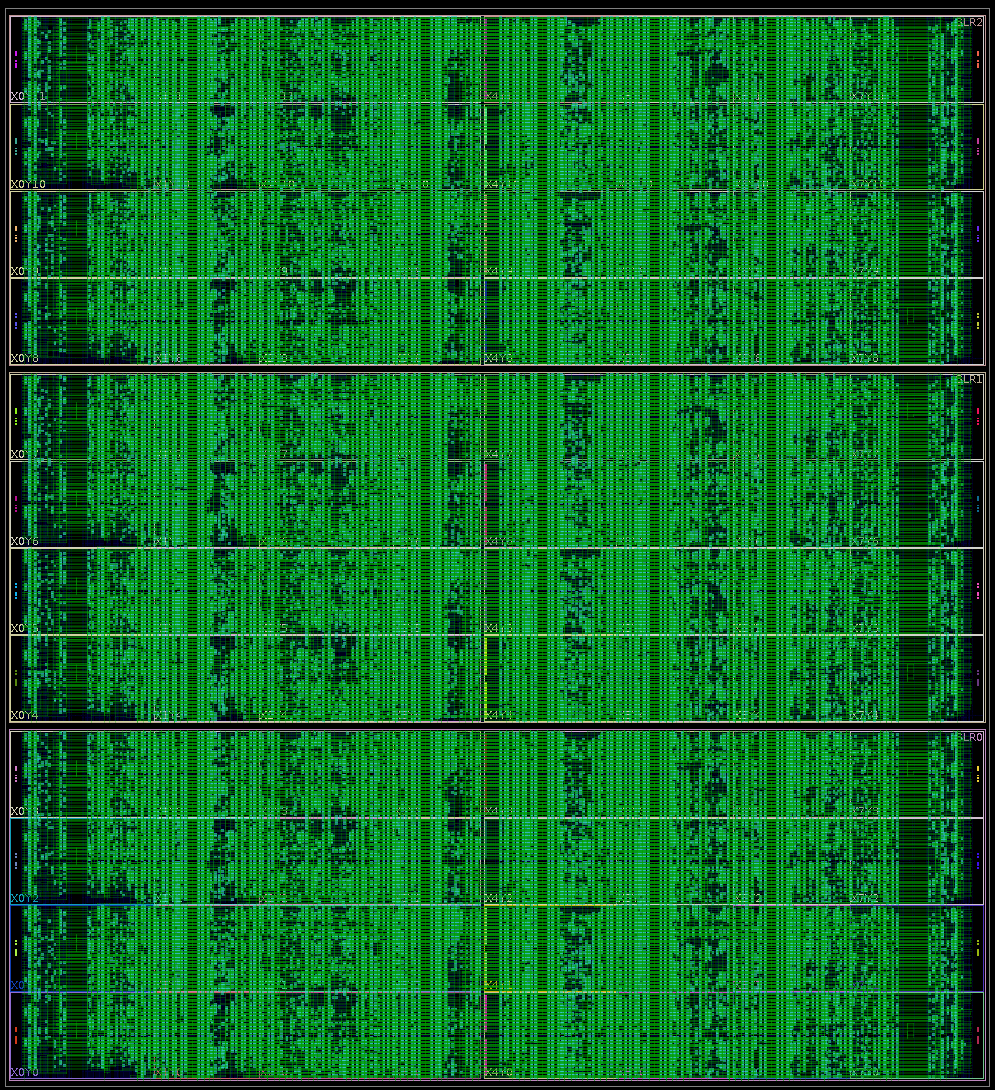
\includegraphics[width=1\textwidth,height=1.3\textwidth]{img/rapidlayout-placed}
    %   \caption{使用RapidLayout完成布局布线的脉动阵列神经网络加速器}
    % \end{figure}

    \begin{figure}[h]
      \centering
      \subfloat[Vivado]{
        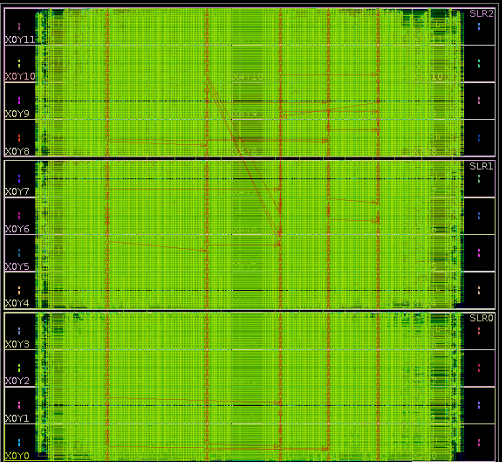
\includegraphics[width=0.5\textwidth, height=0.8\textwidth]{img/vivado-placed.png}
      }
      \subfloat[RapidLayout] {
        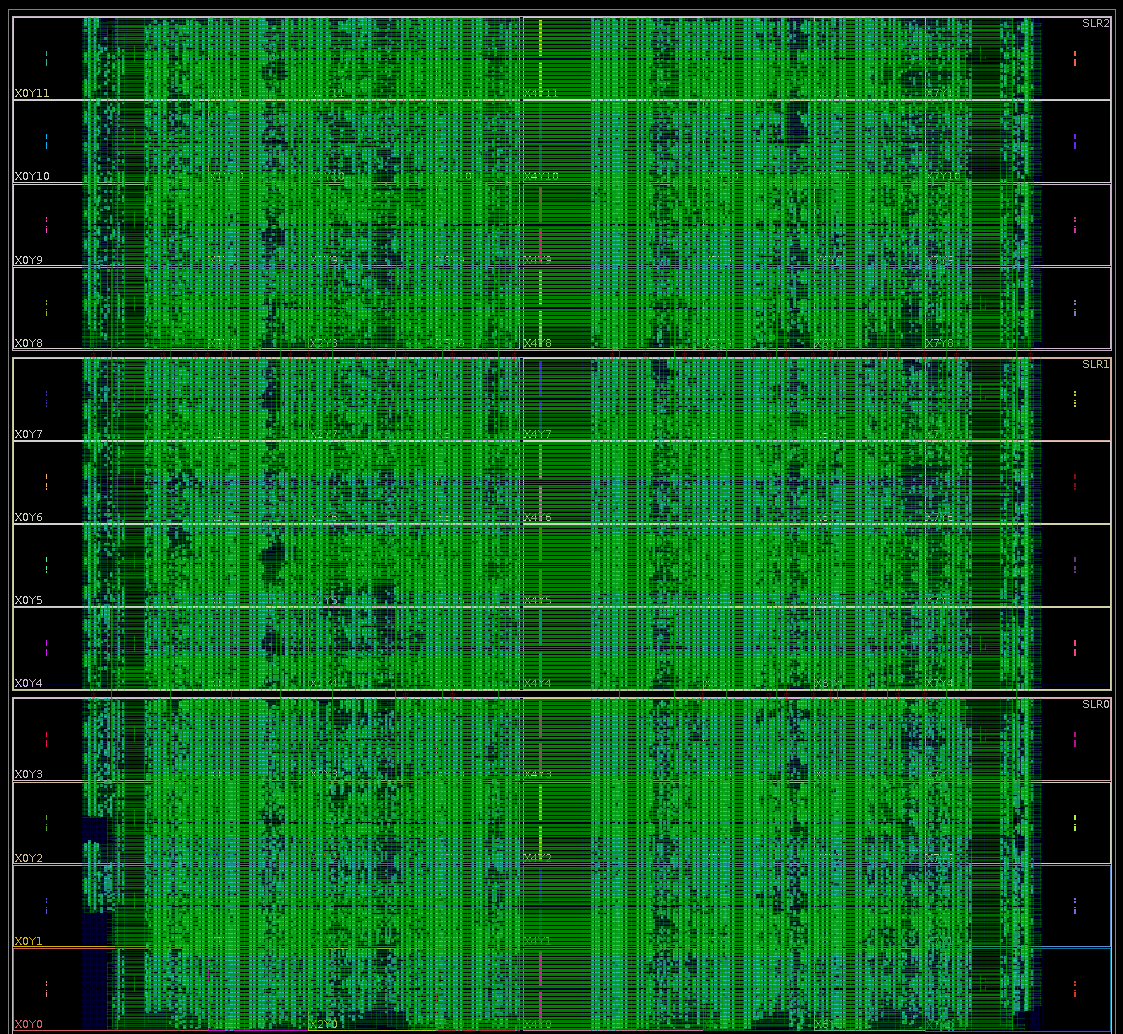
\includegraphics[width=0.5\textwidth, height=0.8\textwidth]{img/manual-placed.png}
      }
      \caption{
       A Successful and Faster Placement Process by RapidLayout
      }
      \label{fig:overview}
    \end{figure}


  \end{columns}

\end{frame}



% \section{附录}

% \begin{frame}{异构FPGA硬核列分布资源}
%   \begin{figure}
%     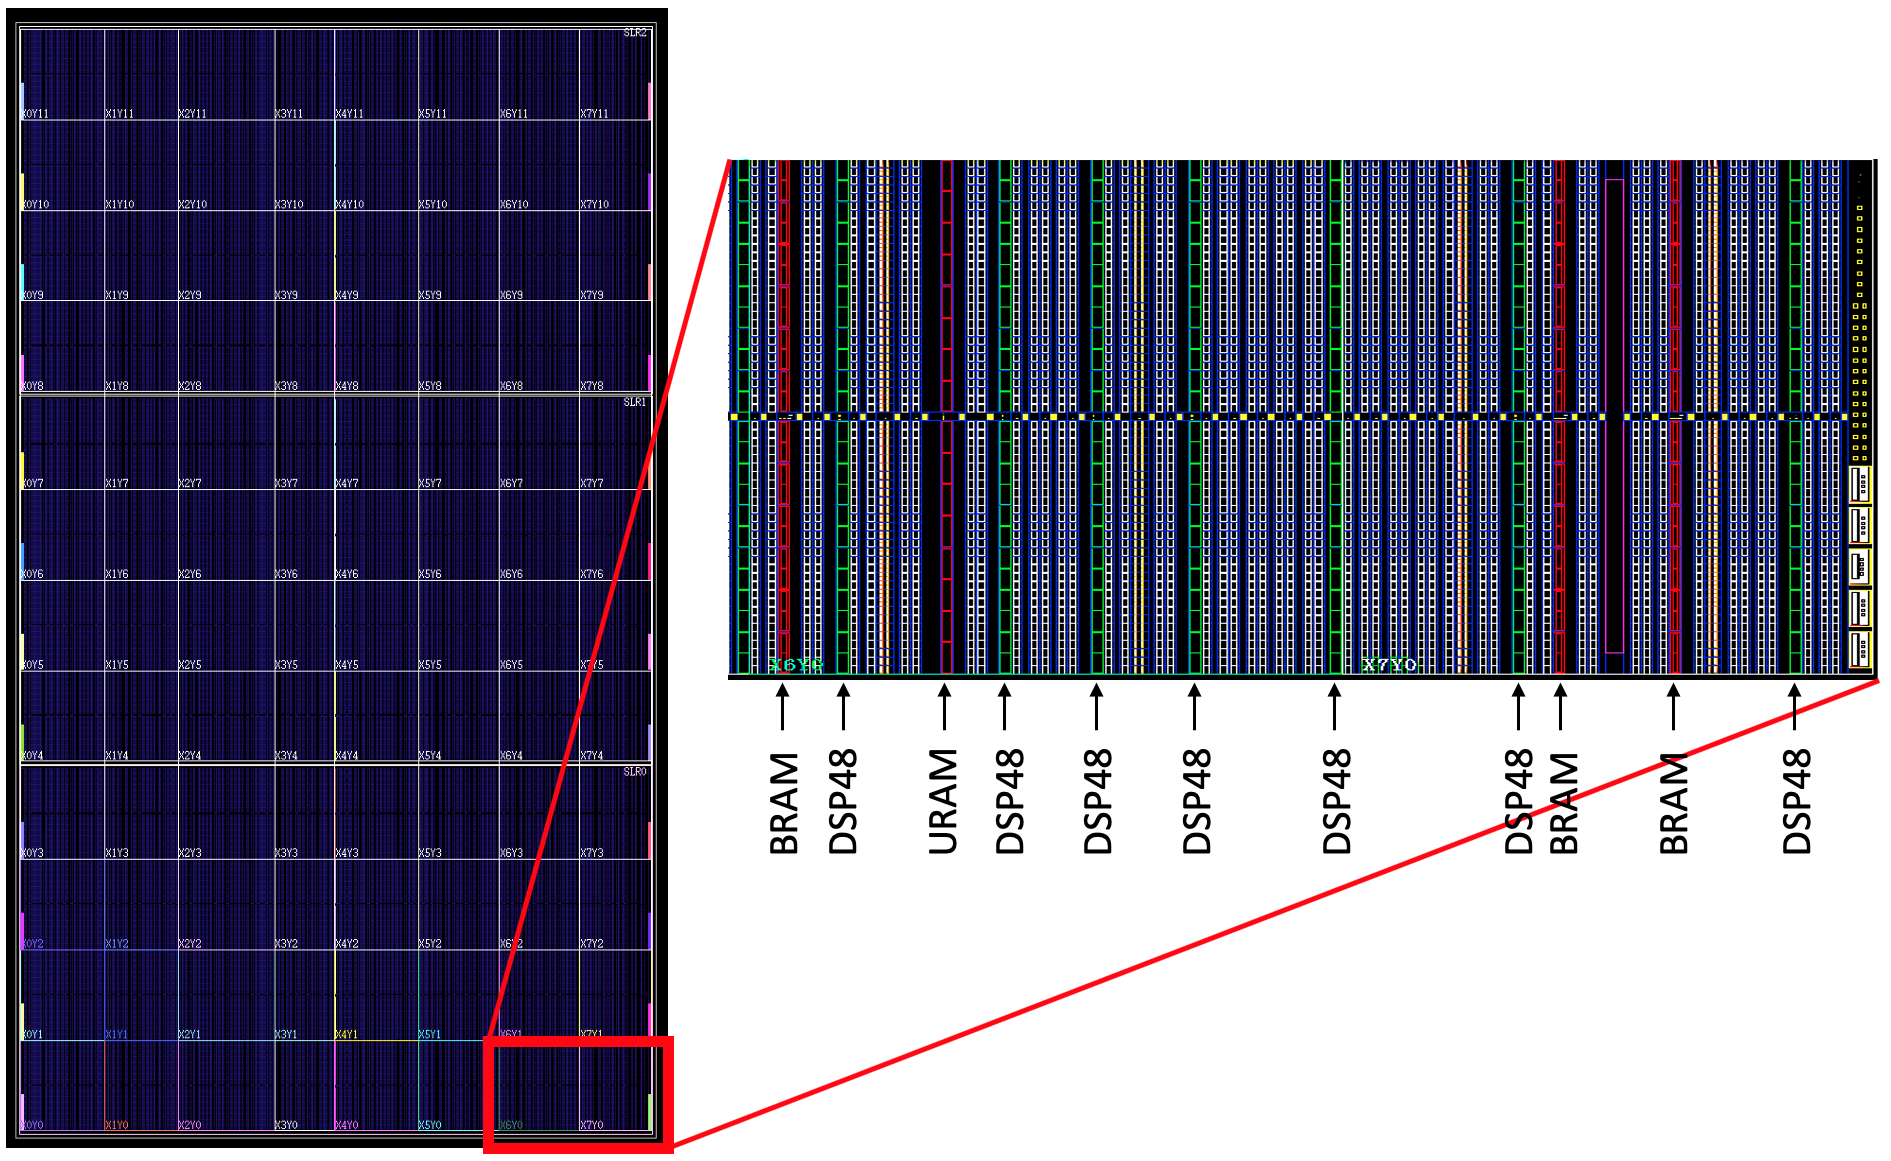
\includegraphics[width=\textwidth]{img/architecture.png}
%   \end{figure}
% \end{frame}


\end{document}
